%%%%%%%%%%%%%%%%%%%%%%%%%%%%%%%%%%%%%%%%%%%%%%%%%%%%%%%%%%%%%%%%%%%
%                                                                 %
%   KUIP  - Reference Manual -- LaTeX Source                      %
%                                                                 %
%   Chapter 3: Programmer Interface                               %
%                                                                 %
%   External EPS files referenced: kuipc.eps                      %
%                                                                 %
%   Editor: Michel Goossens / CN-AS                               %
%   Last Mod.: 10 Dec  1992   mg                                  %
%                                                                 %
%%%%%%%%%%%%%%%%%%%%%%%%%%%%%%%%%%%%%%%%%%%%%%%%%%%%%%%%%%%%%%%%%%%

\chapter{Programmer interface}
%
%---------------------------------------------------------------------------
%

The key to building a user interface with \KUIP{} is the Command
Definition File~(\CDF{})
which the application write has to provide. 
As the name already indicates the \CDF{} defines the available commands
and their grouping into menus.
The \CDF{} directives for the basic \KUIP{} command line interface are
described in section~\ref{basic-CDF}.

Section~\ref{Motif-CDF} introduces the main concepts of \KUIPMotif{}
and describes the \CDF{} directives specific to this interface, e.g.\ how
to add new object types to the browser. 

The \CDF{} is a text file which has to be passed through the \KUIP{}
compiler (\KUIPC{}). 
\index{CDF!compilation}
The output of \KUIPC{} is either Fortran or C source code for a subroutine
which the application program has to call at initialization time in
order to store the \CDF{} information in memory.
\if0
Section~\ref{running-KUIPC} explains how to run \KUIPC{} and the pros and
cons of generating Fortran vs.\ C~source code.
\fi

Figure~\ref{FIG8} shows the steps from the \CDF{} to the running application.
 
\begin{figure}[tb]
\begin{center}
\fbox{\epsfig{figure=kuipc.eps,height=12cm}}
%\fbox{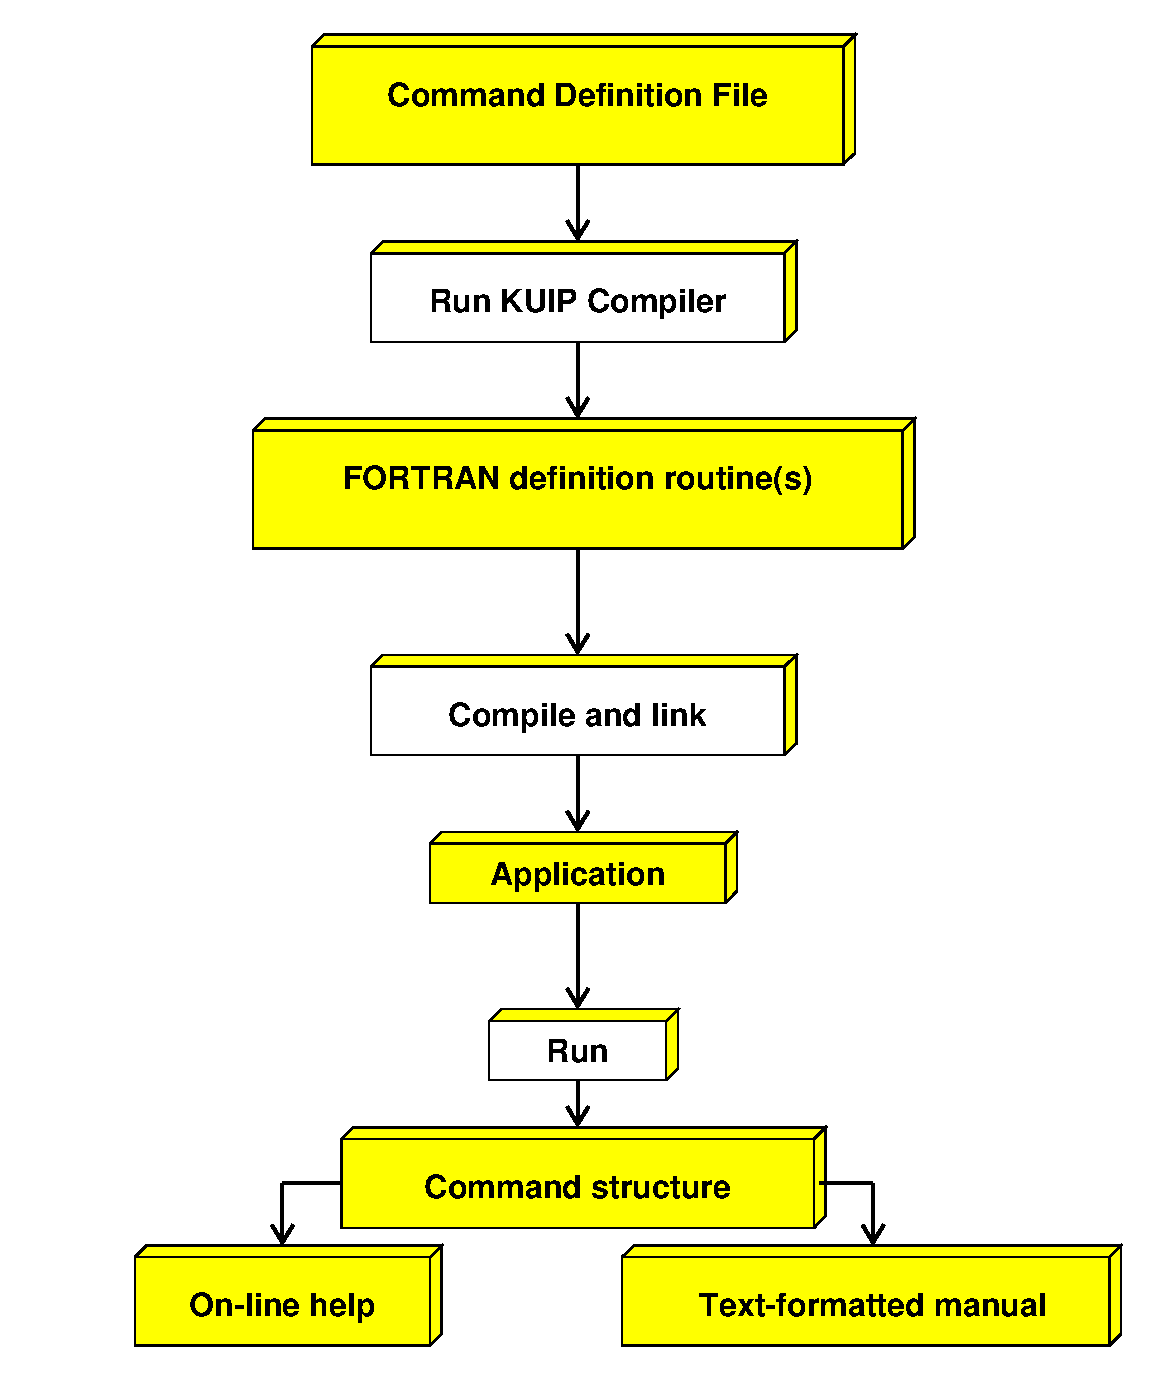
\epsfig{%bbllx=22mm,bblly=30mm,bburx=210mm,bbury=263mm,%
%              file=kuipc.eps,height=12cm}}
\end{center}
\caption{Building an application starting from the \CDF{}.}
\label{FIG8}
\end{figure}

\section{The Command Definition File}

The \CDF{} format is line-oriented.
Completely blank lines are ignored.
An underscore character at the end of a line acts as
continuation symbol, i.e.\ before processing
\index{CDF!continuation lines}
the following line is concatenated to the current line removing the
underscore itself.

Directives
\index{CDF!directives}
starts with a ``\Lit{>}''~character in the first column
immediately followed by the directive name.
Most directives take arguments following on the same line and some
directives expect additional information on separate lines.
\CDF{} argument lines are tokenized according to the rules:
\index{CDF!arguments}
\begin{UL}
\item
Individual arguments must be separated by one or more blanks.
\item
Strings containing blanks must be delimited by single quote characters,
e.g.\ \Lit{'Hello world'}.
\item
Single quote characters inside a string must be duplicated,
e.g.\ \Lit{'N''th value'}.
\item
A single ``\Lit{.}'' is the place-holder for a null argument.
\end{UL}

Names for menus, commands, and parameters
\index{Names}
are case-insensitive and may consists of letters,
digits, minus signs and underscores.
For obvious reasons names containing only digits, starting with a
minus sign, or ending in an underscore should be avoided.
Names may start with a digit.

\section{\CDF{} directives for command definitions\label{basic-CDF}}

The \CDF{} has to define the command tree structure which can contain
three types of elements: 
\begin{UL}

\item
Menus 
\index{menu!definition} 
are the branches of the tree.
Each menu should provide a help text to give general information
about the commands and sub-menus linked to it.

\item
Commands 
\index{command!definition} 
are the terminal leaves of the tree.
The \CDF{} should contain the help text and define the parameters 
(if any).
Each command definition must specify the action routine 
\index{action routine} 
which retrieves the command arguments and performs the intended operations.

\item
Help items \index{help item!definition} are like commands without
action routine. 
Their sole purpose is to provide additional help not related to a
specific command or menu.
Trying to execute a help item is equivalent to asking \Lit{HELP} on that item.

\end{UL}

\condbreak{5\baselineskip}
\begin{Gray}{i}
>* comment
   ...
\end{Gray}
\begin{Gray}{i}
*  comment
\end{Gray}
The \Lit{>*}~directive starts a block comment.
Everything up to the next \CDF{} directive is ignored.
A single line comment is introduced by a ``\Lit{*}''~character in the
first column. 


\begin{Gray}{i}
>NAME  definition-routine
\end{Gray}
The \Lit{>Name} directive defines the name of the routine which
\KUIPC{} will generate, i.e.\ \textsl{definition-routine} must be an acceptable
Fortran \Lit{SUBROUTINE} name.
The application has to \Lit{CALL }\textsl{definition-name} at initialization time
in order to store the command definitions in internal memory.


The first non-comment line in the \CDF{} must always be a \Lit{>Name}
directive. 
The \CDF{} may contain several \Lit{>Name} directives.

\begin{figure}[p]
\begin{XMPtext}{Example for the creation of menus}{
In this example \Lit{CALL KUIPDF} creates the menus \Lit{/KUIP},
\Lit{/KUIP/ALIAS}, \Lit{/KUIP/SET\_SHOW}, and \Lit{/MACRO} and 
\Lit{CALL VECDEF} creates the menu \Lit{/VECTOR}.
}
>Name KUIPDF
>Menu KUIP
>Guidance
      ...
>Menu ALIAS
>Guidance
      ...
>Menu ../SET_SHOW
>Guidance
      ...
>Menu /MACRO
>Guidance
      ...
>Name VECDEF
>Menu VECTOR
>Guidance
      ...
\end{XMPtext}
%\end{figure}
\vspace{-2\baselineskip}
%\begin{figure}[p]
\begin{XMPtext}{Example for the creation of commands}{
In this example the commands \Lit{/KUIP/HELP},
\Lit{/KUIP/ALIAS/CREATE}, and \Lit{/KUIP/ALIAS/DELETE} are created.
}
>Menu /KUIP
>Command HELP
      ...
>Menu ALIAS
>Command CREATE
      ...
>Command DELETE
      ...
\end{XMPtext}
%\end{figure}
\vspace{-2\baselineskip}
%\begin{figure}[p]
\begin{XMPtext}{Example for the creation of a help item}{
This example creates the help item \Lit{/KUIP/FUNCTIONS}.
}
>Menu /KUIP
>Help_item FUNCTIONS
>Guidance
      ...
\end{XMPtext}
\end{figure}

\begin{figure}[p]
\XMPvinput{Example for a guidance text}{xguidance.cdf}{}
\end{figure}

\begin{figure}[p]
\XMPvinput{Resulting HELP menu}{xguidance.hlp}{}
\XMPinput{Formatted output for ``MANUAL MYMENU -LATEX''}{xguidance.tex}{}
\end{figure}

\begin{figure}[p]
\XMPvinput{Example for a user help routine}{xuserhelp.f}{}
\XMPvinput{Terminal output for ``HELP MYMENU''}{xguidance.txt}{}
\end{figure}


\begin{Gray}{i}
>MENU  menu-path
\end{Gray}
Commands are linked into the current menu and the \Lit{>Menu}
directive allows to changes the menu path. 
The \textsl{menu-path} can consist of several components separated
by~``\Lit{/}''. 
The path is relative to the previously valid path unless \textsl{menu-path} starts with a~``\Lit{/}''.
The pseudo-name~``\Lit{..}'' refers to the parent menu.


The names for already existing menus may not be abbreviated.
If a menu is not already existing it is created and should be followed
by a \Lit{>Guidance} directive.

The \Lit{>Name} directive resets the path to the root
menu~``\Lit{/}''. 
Commands and help item should not be linked directly to the root menu.
Therefore the \Lit{>Name} directive should always be a followed by a
\Lit{>Menu} directive. 


\begin{Gray}{i}
>COMMAND  command-name
\end{Gray}
The \Lit{>Command} directive appends a new command to the
current menu.
The \textsl{command-name} must be a bare name without menu path.

The \Lit{>Command} directive must be followed by \Lit{>Guidance} and
\Lit{>Action} directives and can be followed by \Lit{>Parameters} and
\Lit{>User_help} directives in any order.


\begin{Gray}{i}
>HELP_ITEM  help-item-name
\end{Gray}
The \Lit{>Help_item} directive appends a new help item to the
current menu.
The \textsl{help-item-name} must be a bare name without menu path.
The \textsl{help-item-name} cannot contain a menu path.

The \Lit{>Help_item} directive must be followed by a \Lit{>Guidance}
directive and can be followed by a \Lit{>User_help} directive in any order.

\condbreak{2cm}
\begin{Gray}{i}
>GUIDANCE
   text
   ...
\end{Gray}
The \Lit{>Guidance} directive defines the help text attached to the
most recent command tree element created by a \Lit{>Menu},
\Lit{>Command}, or \Lit{>Help\_item} directive.
The help text ends at the next \CDF{} directive.
The formatting rules applied for terminal output and by the 
\Lit{MANUAL} command in \LaTeX{} mode are explained in the example below.


\begin{Gray}{i}
>USER_HELP  user-help-routine
\end{Gray}
The \Lit{>User_help} directive may follow a \Lit{>Command} or
\Lit{>Help_item} directive.
The \textsl{user-help-routine} is called by the \Lit{HELP} command and
allows to add runtime dependent information at the end of the static
\Lit{>Guidance} text. 

The routine has to call \Lit{KUHELP} in order to obtain the 
logical unit where the additional help information should be written to.
The second argument of \Lit{KUHELP} returns the command or help item
name for which \Lit{HELP} was requested.

\begin{Gray}{i}
>PARAMETERS
  mandatory-parameters
+
  optional-parameters
++
  constant-parameters
\end{Gray}
The \Lit{>Parameters} directive heads the parameter definition for a command.
The lines following up to the next directive must be parameter
definitions of the form

\indent\indent\begin{tabular}{llll}
\textsl{parameter-name} & \textsl{prompt-string} & \textsl{parameter-type}
& $[$ \textsl{attribute-list} $]$
\end{tabular}
\vskip\parskip

The underscore continuation has to be used if the complete definition
does not fit onto a single single.
Mandatory and optional parameters are separated by a control line
containing only a ``\Lit{+}''~character in the first column.
If there are only mandatory parameters the ``\Lit{+}''~line is not
required.


Non-positional arguments can be specified
in a command line as \textsl{parameter-name}{\tt=}\textsl{value}.
To allow abbreviations for \textsl{parameter-name} the minimum length has
to be indicated by a ``\Lit{*}''~character, e.g.\
\begin{XMP}
DIR*ECTORY \quad 'Directory path' \quad C
\end{XMP}
defines a parameter \Lit{DIRECTORY} which can be assigned in a command
line as ``\Lit{DIR=}\textsl{value}''.

The \textsl{prompt-string} is used to prompt for missing mandatory
arguments and as labels in the \Motif{} command panel.
Possible \textsl{parameter-type} values are ``\Lit{C}''~for character
strings, ``\Lit{I}''~for integer numbers, and ``\Lit{R}''~for real
numbers.

The \textsl{attribute-list} for mandatory parameters can be empty.
For optional parameters it must specify at least the default attribute:
\begin{XMP} 
D=\textsl{default-value}
\end{XMP}
For mandatory parameters the default value is only used when prompting
for missing arguments and the reply is an empty line.
The default value for optional parameters is passed to the action
routine whenever the argument is missing or given as~``\Lit{!}'' on
the command line.

For all parameter types~\Lit{C}, \Lit{I}, and~\Lit{R} the range
attribute defines a comma-separated list of valid values:
\begin{XMP} 
R=\textsl{value-1},\textsl{value-2},...\textsl{value-n}
\end{XMP}
e.g.\
\begin{XMP} 
PRIME \quad 'Prime number below 10' \quad I \quad R=2,3,5,7
\end{XMP}
For option parameters there is an alternative way to specify the list
of valid values together with an explanation text for each option (see below).
For the numeric parameter types~\Lit{I} and~\Lit{R} the range
attribute can have the form
\begin{XMP} 
R=\textsl{lower-limit}:\textsl{upper-limit}
\end{XMP}
to limit valid values to the interval including the boundaries.
Either the \textsl{lower-limit} or the \textsl{upper-limit} may be
omitted to indicate an unlimited interval in one direction.

Numeric parameters with a limited range are displayed with a slider in
the \Motif{} command panel.
The slider step size for type~``\Lit{R}'' parameters is determined by
the number of digits following the decimal point in the range
definition, e.g.\
\begin{XMP} 
PROB*ABILITY  'Detection probability'  R  D=0.5  R=0:1.00
\end{XMP}
creates a slider for the values 0.00, 0.01, ..., 1.00.
If the range is unlimited or too large the \Lit{Slider} attribute
\begin{XMP} 
SLIDER=\textsl{lower-limit}:\textsl{upper-limit}
\end{XMP}
allows to define a restricted range which affects the slider only.
E.g.\
\begin{XMP} 
EFF*ICIENCY  'Reconstruction efficiency'  R  R=0:1  Slider=0.900:1
\end{XMP}
creates a slider for the values 0.900, 0.901, ..., 1.000.

\begin{figure}[tb]
\XMPvinput{Example for option parameter definitions}{xparameter.cdf}{}
\end{figure}

\begin{figure}[tb]
\XMPvinput{Argument assignments for command ECHO}{xparameter.log}{}
\end{figure}

%\begin{figure}[tb]
%\XMPvinput{Terminal output for ``HELP ECHO''}{xparameter.txt}{}
%\XMPinput{Formatted output for ``MANUAL ECHO -LATEX''}{xparameter.tex}{}
%\end{figure}

The \Lit{Option} attributes defines a parameter to be an option for
which ``\Lit{-}\textsl{value}'' can be used to specify non-positional
option arguments on the command line.
The \Lit{Option} attribute is set implicitly
if \textsl{parameter-name} begins with \Lit{OPTION} or \Lit{CHOPT}.
The ``\Lit{-}''~mechanism requires a range definition including all
valid option values.
The list of option values is defined by lines
\begin{XMP} 
-\textsl{option-value} \quad \textsl{explanation-text}
\end{XMP}
following the option parameter definition itself.
The ``\Lit{-}''~character must be in the first column and is not part
of the option value.
The underscore continuation has to be used if the complete 
\textsl{explanation-text} does not fit onto a single single.
The rules applied for formatting the list of options as a table are
explained in the example. 

A command can contain contain several option parameters as long as the
option values are distinct.
Option values can be specified with the range attribute
if an \textsl{explanation-text} is not required.
Blank is permitted as \textsl{option-value} but cannot be combined with
any other value.
Consequently it should only be used if all option values are mutually
exclusive, and it should be the default value.

The interpretation of a ``\Lit{-}\textsl{value}'' argument as option
is considered only if \textsl{value} consists
exclusively of valid values from a single option parameter.
In some instances ``\Lit{-}\textsl{value}'' is intended be a positional
argument even though it could match an option parameter as well.
It depends then on the definition of the parameter which
should be assigned next whether the argument is actually interpreted
as option ``\textsl{value}''.

If ``\Lit{-}\textsl{value}'' can be interpreted as a negative number
and the next parameter is numeric the option assignment is inhibited.
A character parameter can be given the \Lit{Minus} attribute to
indicate that arguments at its position should never be assign to an
option parameter.

The leading ``\Lit{-}'' is usually stripped off in an option
assignment. 
Only in case the next argument position belongs to the option
parameter itself and ``\Lit{-}'' is one of its option values
it is passed on to the action routine.
In order to avoid confusion due to this position dependence digits and
the minus sign should not be used as option values.


It is often desirable for a command to be able to accept a
variable-length list of values for one of the parameters.
If the command operation is independent for each list item
the \Lit{Loop} attribute can be added to the corresponding parameter
definition.
For a comma-separated argument list the action routine is then called
repeatedly passing it the next list item each time.
E.g.\ with the definition
\condbreak{1cm}
\begin{XMP}
>Command DELETE
>Parameters
LIST  'List of items'  C \quad Loop
\end{XMP}
the command line
\begin{XMP}
DELETE x,y,z
\end{XMP}
is equivalent to
\begin{XMP}
DELETE x ;  DELETE y ;  DELETE z
\end{XMP}
and the action routine only needs to handle a single item.
A ``\Lit{,}'' inside a quoted string or an unbalanced set of
parentheses is not treated as item separator, i.e.\ ``\Lit{'foo,bar'}''
and ``\Lit{xyz(3,4,5)}'' are single items only.

In case the action routine needs access to all list items it can call
\Rind{KUGETL} to retrieve the items one by one.
The \Lit{Vararg} attribute can be given to a list parameter if it is
the last one of the command. 
This allows to use \Rind{KUGETL} also for a blank separated item list,
i.e.\ with the definition
\begin{XMP}
>Command ASSIGN 
>Parameters 
ARRAY  'Array name'  C 
VALUES  'List of values'  C  Vararg
\end{XMP}
both command line forms
\begin{XMP}
ASSIGN  name  foo,bar 
ASSIGN  name  foo  bar
\end{XMP}
can be handled by the same action routine.

In \Motif{} mode the arguments entered in the command panel are usually
treated as a single value, i.e.\ if they contain a blanks they are
implicitly quoted.
In some cases, for example the macro arguments passed in the
\Cind{EXEC} command, this behavior must be inhibited.
The \Lit{Separate} attribute allows to flag the last parameter that
the value entered in the \Motif{} input field should be interpreted as
separate command line tokens.


\condbreak{3\baselineskip}
\begin{Gray}{i}
>ACTION  action-routine
\end{Gray}
The \Lit{>Action} directive must follow a \Lit{>Command} and defines
the routine which should be called after decoding the command line in
order to perform the intended operations.

\begin{figure}[tb]
\XMPvinput{Example for an action routine}{xecho.f}{}
\end{figure}

An action routine does not have arguments.
The command line arguments have to be retrieved 
by calling the suitable \Lit{KUGET}\textsl{x} routine for each parameter
from inside the action routine.

The same action routine can be used for different commands.
The routines \Lit{KUPATH} and \Lit{KUPATL} allow to identify which
command was actually requested.

\if0
\section{Retrieving parameters in action routines}

Action routines are called automatically by \KUIP{} when the corresponding
command is entered. The application programmer, in addition to defining
their names with the \Command{>Action} keyword in the \CDF{}, will have to write
these action routines and to link them together with the rest of its application.

Inside action routines, parameters, as defined with \Command{>Parameters}
in the \CDF{}, have to be retrieved by calling the
\KUGETx{} routines, e.g.:
\Rind[KUGETI]{KUGETI(IPAR)}, \Rind[KUGETR]{KUGETR(RPAR)}, 
\Rind[KUGETC]{KUGETC(CHPAR,NCH)},\ldots for parameters of the
type Integer, Real and Character type parameters respectively.
%
%---------------------------------------------------------------------------
%
\fi
%
%---------------------------------------------------------------------------
%
\section{Browser Concepts and Definitions}
\label{ref:rebrodef}

The high-light of the \KUIPMotif{} interface is a general-purpose object
browser.
Before going into the details of the \CDF{} directives for customizing
the browser we want to introduce the main concepts and the terminology
used.

The browser allows to traverse a hierarchical directory structure of 
objects. Operations on these objects can be chosen from pop-up menus which
depend on the object type (or ``class'').

To incorporate your own application specific objects into the browser
you have to:
\begin{UL}
\item
describe in the \CDF{} (``Command Definition File'') the object types 
(``classes'') and the containers for these objects (``browsables''),
\item
write ``small'' routines to scan through the list of objects, and 
eventually the list of browsables,
\item
describe in the \CDF{} the action menus for classes of objects and browsables.
\end{UL}

\subsection{Classes of Objects}
\label{ref:recldef}

``Classes'' of objects can be any kind of entities handled by an application.

For example:
\begin{UL}
\item
HIGZ pictures and \HBOOK{} data (1d-histograms, 2d-histograms, 
N-tuples, chains and directories) are ``Classes'' defined in
\PAW++{}.
\item
in Geant++  the classes are the data structures: volumes, materials, 
particles, ...
\item
in \KUIPMotif{} the commands themselves have been defined as classes,
as well as the different type of files (read, read-write, executable,
and macros ...).
\end{UL}

Object classes are defined in the \CDF{} with the directive:
\begin{Gray}{i}
>Class  class-name  menu-title  [ big-icon  small-icon ]
\end{Gray}

\begin{figure}[tb]
\begin{PICTf}[.45]{pkmf15}
\begin{DLsf}{}
\item[\quad \CDF{} description (extract) :]
\item
\item
\begin{XMPt}{Example of the ``Class'' directive}\footnotesize

>Class 1d 1d-Histogram big_1d sm_1d
 Plot        .  .  default_action%C
'/Fit...'    .  'Histo/Fit [this]'
'Fit Gauss'  .  'Histo/Fit [this] G'
'Fit Exp'    .  'Histo/Fit [this] E'
'Fit Const'  .  'Histo/Fit [this] P0'
'Fit Linear' .  'Histo/Fit [this] P1'
 /Smooth     .  'Smooth [this]'
'Smooth...'  .  '-Smooth [this]'
 /Copy       .  'Histo/Copy [this]'
 Reset       .  'Histo/Op/Reset [this]'
!Delete      .  'Hio/Hscratch [this]'
+
...
\end{XMPt}
\end{DLsf}
\end{PICTf}
\begin{EnumZB}
\item Icon used to represent the object class ``1d'' (normal size).
\item Action menu (title ``1d-Histogram'') associated to the selected object 
(histogram of class ``1d'' with name/identifier ``10'').
\vspace{-1\baselineskip}
\end{EnumZB}
\caption{Object Classes}
\label{ref:FIGPKMF15}
\end{figure}

E.g.\ The directive ``{\tt >Class 1d '1d-Histogram' big\_1d sm\_1d}'' in the 
\PAW{} \CDF{} is used for 1D histograms : the class name is ``1d'', ``big\_1d''
(normal size) and ``sm\_1d'' (small size) are the icons used by the browser 
for a graphical representation and ``1d-Histogram'' is the title text for
the pop-up menu displayed when object types ``1d'' are selected in the browser
(see figure~\ref{ref:FIGPKMF15}).

\subsection{Browsables}
\label{ref:rebrdef}

All objects are part of container objects constituting the top level directory
(e.g.\ ZEBRA/RZ files.). We will call these containers the ``browsables''.
They are defined with the \CDF{} directive
\begin{Gray}{i}
>Browse  browsable-class  menu-title  scan-objects  [ scan-browsables ]
\end{Gray}

\begin{figure}[tb]
\begin{PICTf}[.5]{pkmf16}
\begin{DLsf}{}
\item[\quad \CDF{} description (extract) :]
\item
\item
\begin{XMPt}{Example of the ``Browse'' directive}\footnotesize

>Browse Commands . kscncmds%C
 List
'Set Default'  .  ' Set/Root /'
...
>Class /Menu Menu big_menu sm_menu
...
>Class Cmd Command big_cmd sm_cmd
...
\end{XMPt}
\end{DLsf}
\end{PICTf}
\begin{EnumZB}
\item The browsable ``Commands'' is selected.
\item Action menu corresponding to this browsable.
\item \OW{} with the list of commands (class ``Cmd'') and menus 
(class ``/Menu'') for the current directory ``/KUIP'' \NbDB{4}.
\vspace{-1\baselineskip}
\end{EnumZB}
\caption{Browsables}
\label{ref:FIGPKMF16}
\end{figure}

For example:
\begin{UL}
\item
in \PAW++{}, a browsable HBOOK (see figure~\ref{ref:FIGPKMF16}) has been
defined, which is a container for any  
kind of \HBOOK{} data (1d/2d histograms and Ntuples).
\item
in \KUIPMotif{}, the browsable ``Files'' contains and displays all files
(read, read-write, executables, and \KUIP{} macros). Another browsable 
``Commands'' has been defined for all the commands and menus defined 
by \KUIP{} and the application.
\end{UL}

For a detailed description of the ``{\tt >Class}'' and
``{\tt >Browse}'' \CDF{} directives see sections~\ref{ref:recdfobj} 
and~\ref{ref:recdfbro}.

\subsection{The ``scan-objects'' routine}

To make the objects belonging to one browsable for a given path (directory)
accessible by the browser, the application has to provide a scanning routine 
which, when called for the first time, returns the first object and
subsequently returns the next object until no more objects are left: this
is what we have called the ``scan-objects'' routine in the \CDF{} directive 
for the browsable definition. The browser passes to this routine the 
identification of the requested subdirectory and expects in return:
\begin{UL}
\item
the object name, e.g.: 
\begin{UL}
\item
for ``{\tt >Browse HBOOK}'' in \PAW++{}: the histogram or Ntuple identifier 
(number).
\item
for ``{\tt >Browse Commands}'' in \KUIPMotif{}: the menu or command name.
\end{UL}
\item
the object class, e.g.: 
\begin{UL}
\item
for ``{\tt >Browse HBOOK}'' in \PAW++{}: ``1d'', ``2d'' or ``Ntuple'' 
(assuming that ``{\tt >Class 1d}'', ``{\tt >Class 2d}'' and 
``{\tt >Class Ntuple}'' have been defined).
\item
for ``{\tt >Browse Commands}'' in \KUIPMotif{}: ``Menu'', ``Cmd'' and ``InvCmd''
(assuming that ``{\tt >Class Menu}'', ``{\tt >Class Cmd}'' and 
``{\tt >Class InvCmd}'' have been defined).
\end{UL}
\item
and eventually a short and a long description text (title) of this object 
(which will be used to display the list of objects in various forms: big icons, 
small icons, text only).
\end{UL}
This ``scan-objects'' routine can be coded in Fortran or in~C. 

\subsection{The ``scan-browsables'' routine}

We have to make a distinction between two kinds of browsables:
\begin{UL}
\item
``single instance'' browsables,
\item
or ``multiple instances'' browsables.
\end{UL}
A ``multiple instances'' browsable gives the possibility to have several
instances of the same browsable. For instance, in \PAW++{}, the browsable
``{\tt >Browse HBOOK}'' which is defined for the ZEBRA/RZ files, acts as a
container for the objects 1d/2d histograms and Ntuples. As it is
possible to have several ZEBRA/RZ files opened at the same time and 
connected to different logical units (LUN), the browsable HBOOK has been
defined as a ``multiple instances'' one. This is done by providing
a second scanning routine from which the name of all the currently connected
instances of a given browsable can be retrieved (e.g.\ for all the ZEBRA/RZ 
files opened and connected to some logical unit  the name is a concatenation
of ``LUN'' and this number, i.e.\ ``LUN8'' for logical unit 8).
This is what we have called the ``scan-browsables'' routine  (optional for a 
``single instance'' browsable) in the \CDF{} directive for the browsable 
definition.

This ``scan-browsables'' routine can be coded in Fortran or in~C.

Note that ``single instance'' browsables are always displayed in the 
browser (as soon as it is created) whereas ``multiple instances''browsables
can be accessed and displayed at run time (e.g.\ in \PAW++{} when a new 
ZEBRA/RZ file is opened).

For a more precise description of the the calling sequence of the 
``scan-objects'' and ``scan-browsables'' routines see section 
\ref{ref:recdfbro}.

\subsection{Directories}

A tree structure of objects can easily be achieved by defining a special class
for subdirectories of a browsable. The corresponding \CDF{} directive 
is the same 
as for simple object classes, ``{\tt >Class}'', except that there must a 
``{\tt /}'' in front of the class name.

For example:
\begin{UL}
\item
in \PAW++{}, ZEBRA/RZ directories (browsable ``HBOOK'') are ``directories''
classes of objects: 
\begin{XMPt} {}
       >Class /dir Directory big\_dir sm\_dir
\end{XMPt}
Ntuple chains (in the ``Chains'' browsable) are also defined as a ``directory'' 
class of objects:
\begin{XMPt} {}
       >Class /chain Chain big\_chain sm\_chain
\end{XMPt}
\item
in \KUIPMotif{} the menus (in the ``Commands'' browsable) are defined as 
a ``directory'' class of objects:
\begin{XMPt} {}
       >Class /Menu Menu big\_menu sm\_menu
\end{XMPt}
This is also true for directories of files (in the ``File'' browsable):
\begin{XMPt} {}
       >Class /DirFile Directory big\_menu sm\_menu
\end{XMPt}
\end{UL}

This ``special'' class of objects obeys to certain rules:
\begin{UL}
\item
The first item in the action menu is always ``List'' and means ``switch into 
this subdirectory''. Selecting this item (automatically performed with 
a <double click> with the left button) has the effect to update
the content of the \OW{} with the list of objects contained
into the new subdirectory.
\item
The entry ``Path:'' (Fig. \ref{ref:FIGPKMF16}, 
\NbDB{4}) is automatically updated
with the new directory path, which is formed by concatenating the previous
path, a ``{\tt /}'', and the name of the directory object selected.
Going upwards in the directory hierarchy is done by selecting a
substring of the current path displayed in this text entry. Clicking
a second time on the same path segment performs the directory change
and updates the \OW{} in the same way as selecting the ``List'' 
menu entry for a directory object.
\end{UL}

\subsection{Action menus}

For each class of objects it is possible to define two menus which describe 
possible actions if an object of this class is selected:
\begin{UL}
\item[(1)]
either in the browser \OW{},
\item[(2)]
or identified inside a HIGZ \GW{} (if any).
\end{UL}

\condbreak{3\baselineskip}
For each browsable it is possible to define:
\begin{UL}
\item[(3)]
one menu which describes possible 
actions if this browsable is selected (\BW{}), 
\item[(4)]
for ``multiple instances'' browsables, a second menu which describes 
the actions required to connect or de-connect one instance of this 
browsable at run time (menu ``File'' in the \MB{}).
\end{UL}

Menus (1), (2) and (3) pop up when pressing the right mouse button 
in the corresponding window, and the
selected action is performed when the button is released. A <double click>
with the left mouse button on one specific object or on one specific 
browsable always executes the first menu item. Menu (4) is accessed by 
selecting the entry ``File'' in the \MB{} menu-bar.

Object and browsable specific action menus are derived from sequences of action 
definitions written in the \CDF{} and following the {\tt >Class} or 
{\tt >Browse} directive (Fig. \ref{ref:FIGPKMF15} and \ref{ref:FIGPKMF16}). 
For a precise description of the syntax and behavior 
of the \CDF{} directives for action menus see section \ref{ref:recdfacm}.


\section{\CDF{} directives for \KUIPMotif{}\label{Motif-CDF}}

\label{ref:recdf}

We will describe in this section the new \CDF{} (Command Definition File)
directives which have been introduced in \KUIPMotif{}. Please note that
these new directives have to be used only to take advantage of the MOTIF
style and to include your application specific objects into the interface
(and especially into the browser(s)). BUT one must be aware that IT IS 
POSSIBLE to get a \Motif{} interface for any \KUIP{} based application 
WITHOUT modifying the \CDF{}, but only modifying very slightly the 
application main program in order to give control to the ``\Motif{} main loop'' 
(i.e.\ call KUWHAM instead of KUWHAT or KUWHAG).

In all the directives we will describe the square brackets (``[]'') mean
that the corresponding entity is optional: either some default value
is automatically provided if it is missing (e.g.\ for titles), or the
entity is not necessary requested. If such an optional entity happens
to be in the middle of the directive (not at the end) then it has
to be replaced by a ``.'' if no real value is given.

We advice users who want to take advantage of the \Motif{} style to compile 
their \CDF{}s into C~code (instead of Fortran): this is automatically 
performed by the \KUIPC{} compiler when giving the extension ``\Lit{.c}'' to the 
output file which is produced.

N.B. It is preferable to separate the directives for the usual command mode
interface and the directives specific to the \Motif{} style (objects, browsables
and action menus definitions) into different \CDF{}s. Then it will be easy
and possible to make the same application work on a dumb terminal (offering 
only the \KUIP{} command mode interface) or on a \Motif{} workstation, with only 
very few differences in the application main program. 

\subsection{For Classes of Objects}
\label{ref:recdfobj}

As we have already seen (section \ref{ref:recldef}), classes of objects 
are defined in the \CDF{} with the directive
\begin{Gray}{i}
>Class  class-name  menu-title  [ big-icon  small-icon ]
\end{Gray}
for example,
\begin{XMP}
>Class ExFile 'Executable File' big_fx sm_fx
\end{XMP}

The ``menu-title'' should be a short explanation concerning the class (or type)
of object and is used as a title text for the action menu which is displayed
when one object of this class is selected (either in the browser, or in the
\GW{} if any). If no title is given the ``class-name'' is used 
instead. 

``big-icon'' and ``small-icon'' are the names for the icons representing 
graphically this class of object inside the browser. Default icons are
provided if these values are missing, but then the same iconic representation
will be used for all object classes. It is a lot better to have a different
representation for each object class. To create a new icon bitmap you can use
the X11 standard bitmap editor. The icons definitions in the \CDF{} follow
the directive {\tt >Icon\_bitmaps} (see \ref{ref:rebmdef}).


\subsection{For Browsables}
\label{ref:recdfbro}

As we have seen in section \ref{ref:rebrdef}, browsables are defined with the 
\CDF{} directive
\begin{Gray}{i}
>Browse  browsable-class  menu-title  scan-objects  [ scan-browsables ]
\end{Gray}
for example,
\begin{XMP}
>Browse Macro . kmbmac%C kmbmdi%C
\end{XMP}

The ``menu-title'' should be a short explanation on the browsable itself
and is used as a title text for the action menu which is displayed
in the browser ``FileList'' window when this browsable is selected. If a 
``.'' is put instead, then the browsable-class becomes by default the 
menu-title.

\subsubsection{The ``scan-objects'' Routine}
\label{ref:recdfsco}

The ``scan-objects'' routine can be written in Fortran or in~C. 
The browser passes to this routine the identification of the requested 
subdirectory (path) and expects in return: the object name, the class 
name, and eventually a short and a long description text (title) of this 
object. In both cases (Fortran or~C) the calling sequence is predefined. 

In Fortran the calling sequence of the ``scan-objects'' routine 
is the following:
\condbreak{3cm}
\begin{XMPt}{scan-objects routine (in Fortran)}\footnotesize
      SUBROUTINE SCNOBJ(BRNAME,BRCLAS,BRPATH,OBNAME,OBCLAS,STEXT,LTEXT)
      CHARACTER*(*) BRNAME,BRCLAS,BRPATH,OBNAME,OBCLAS,STEXT,LTEXT
*
*            Browser interface to return next object
*
*            Input Parameters  :
*
*                      BRNAME  : browsable name (displayed in the browser)
*                      BRCLAS  : browsable class name (from the ``>Browse'' directive)
*                      BRPATH  : current directory path
*
*            Input / Output    :
*
*                      OBNAME  : object name or identifier
*                                ' ' the first time, previous object otherwise
*
*            Output Parameters :
*
*                      OBCLASS : class name                
*                      STEXT   : short text description of the object
*                      LTEXT   : long text description of the object
*
*     ...
*     IF(OBNAME.EQ.' ') THEN
*        Initialize the scan-objects routine        
*     ENDIF
*     ...
*
      OBCLASS = ...
      STEXT = ...
      LTEXT = ...
*
      END
\end{XMPt}

\condbreak{4cm}

In C the calling sequence is:
\begin{XMPt} {scan-objects routine (in C)}
char **scnobj( brobj_name, brcls_name, bpath, n )
     char *brobj_name;  /* browsable name (displayed in the browser) */
     char *brcls_name;  /* browsable class (from the ``>Browse'' directive) */
     char *bpath;       /* current directory path */
     int n;             /* object position (0 the first time) */
\{
  static char     *obj_desc[4];

    ...
    if (n == 0) \{
       /* Initialize the scan-objects routine */
    \}
    ...

    return obj_desc;   /* obj_desc[0] --> object name or identifier
                          obj_desc[1] --> class name
                          obj_desc[2] --> short text description of the object
                          obj_desc[3] --> long text description of the object
                        */
\}
\end{XMPt}

The browsable name and class-name are identical for ``single instance'' 
browsables. They can be different for ``multiple instances'' browsables.
e.g.\ for ``{\tt >Browse HBOOK}'' in \PAW++{}: the browsable class is ``HBOOK'' 
and the browsable name is ``LUN8'' for a ZEBRA/RZ file connected to logical 
unit 8.

The selected object name (or identifier) and its corresponding long text 
description are printed at the very bottom line of the browser
(\NbDB{6} in Fig.\ref{ref:FIGPKMF9}).

\subsubsection{The ``scan-browsables'' Routine}
\label{ref:recdfscb}

The ``scan-browsables'' routine (optional for ``single instance'' browsables 
but required for ``multiple instances'' ones) can be written in Fortran or 
in~C.  The browser passes to this routine the browsable class-name (e.g.\ 
in \PAW++{}, ``\Lit{HBOOK}'' for ZEBRA/RZ files) and expects in return: the browsable 
name (e.g.\  ``\Lit{LUN8}'' for a ZEBRA/RZ file connected to logical unit~8)
and eventually a string with the description of a predefined set of 
variables concerning this browsable. These variables are used as ``key-words''
in the actions menus connected to the browsables or the classes of objects. 
Some of these variables are fixed by \KUIPMotif{} itself:
\begin{UL}
\item
the variable ``file'' is used to fill the corresponding label (``File:'') 
at the bottom of the browser. 
\item
``root'' is used for setting the path of the top level directory 
(e.g.\ ``\Lit{//LUN8}''),
\end{UL}
The `scan-browsables'' routine for a ``single instance'' browsable can be 
defined just for setting this ``description string'' with the required
key-words.

\condbreak{4cm}

In Fortran the calling sequence of the ``scan-browsables'' routine 
is the following:
\begin{XMPt}{scan-browsables routine (in Fortran)}\footnotesize
      SUBROUTINE SCNBRO(BRCLAS,BRNAME,VARSET)
      CHARACTER*(*) BRCLAS,BRNAME,VARSET
*
*            Browser interface to return next browsable instance
*
*            Input Parameters  :
*
*                      BRCLAS  : browsable class name (from the ``>Browse'' directive)
*
*            Input / Output    :
*
*                      BRNAME  : browsable name (displayed in the browser)
*                                ' ' the first time.
*
*            Output Parameters :
*
*                      VARSET  : set of variables for this browsable.
*
*     First call to this routine 
      IF(BRNAME.EQ.' ') ...
*
      ... 
\condbreak{7\baselineskip}\vspace{-\baselineskip}
      BRNAME = ...
      VARSET='root= ... file= ... ...=...'
      ...
*
      END
\end{XMPt}
E.g.\ in \PAW++{}, for ``{\tt >Browse HBOOK}'' and the browsable ``LUN8'' (ZEBRA/RZ
file connected on logical unit 8) the routine SCNBRO will return something
like:
\begin{XMP}
VARSET = root=//LUN8 file='/user/paw/demo/hrztest.dat'  unit=8
\end{XMP}
In this example ``unit'' is a key-word specific to the browsable HBOOK that 
can be used later on in the action menu definition (e.g.\ ``Close [unit]'').
(See next section \ref{ref:recdfacm} for a complete description of the 
``action menu definition'').

\condbreak{4cm}
In C the calling sequence is the following:
\begin{XMPt} {scan-browsables routine (in C)}
char **scnbro( class_name, first )
     char *class_name;
     int first;
\{
    static char *path_desc[2];

    ...
    if (first) {
       /* First call to this routine */
    }
    ...

    return path_desc;  /* path_desc[0] --> browsable name
                          path_desc[1] --> set of variables for this browsable
                        */
\}
\end{XMPt}

\subsection{For Actions Menus}
\label{ref:recdfacm}

Both the ``{\tt >Class}'' and ``{\tt >Browse}'' directives can be followed 
by sequences of action definitions which obey to the following syntax:
\begin{Gray}{i}
menu-text  [ special-flags ]  [ action-string ]  [ action-routine ]
\end{Gray}
N.B. the components which are missing, when optional (enclosed with ``[]'' 
in the syntax description above), must be replaced by a ``.'' if they are
not the last ones.

The ``menu-text'' is the text that will appear in the pop-up menu. It should
be short but meaningful. ``/'' and ``!'', when they are the very first 
character of this menu-text have special meanings:
\begin{UL}
\item
a ``/'' means that the menu item has to be preceded by a separator,
\item
a ``!'' means that the browser has to be updated when the action is
performed (because the ``objects window'' may have changed).
\end{UL}

The entity ``special-flags'' is not used at the moment and has to be
replaced by a ``.''.

The action can be specified as a string of commands (``{\tt action-string}'')
which should be executed and/or a user-written and application specific 
routine (``{\tt action-routine}'') which should be called. 

In both cases (``{\tt >Class}'' and ``{\tt >Browse}'') two sets of menus 
can coexist and are separated by a blank line starting with the 
character ``+''. The first menu always applies to objects/browsables 
which are identified in the browser. In most cases the
menu pops up when pressing the right mouse button and the selected
action is performed when the button is released.

For the ``{\tt >Class}'' directive the second menu applies to objects which 
are identified in the HIGZ \GW{} if any. (E.g.\ in \PAW++{}, 
``{\tt >Class 1d}'' and ``{\tt >Class 2d}'' histograms can be 
identified either in the browser or in the graphics window: two sets of
menu are then defined in the \CDF{}). 

For the ``{\tt >Browse}'' directive a second menu can be defined to fill 
the ``File'' menu-bar entry in the browser with the list of commands to 
connect or de-connect one instance of a ``multiple instances'' browsable 
(e.g.\ in \PAW++{} open or close a ZEBRA/RZ file containing \HBOOK{} data). 

Only one of the two menu sets can be defined in both cases.

N.B. For graphical object identification inside the graphics window 
please refer to the description of the two HIGZ routines \IGPID{} and
\IGOBJ{} in the HIGZ manual \cite{bib-HIGZ}.

\subsubsection{Action-string (String of Commands)}

When the action is specified as a string of commands,
constructs of the form ``{\tt [}{\em var}{\tt ]}'' can insert
identifications of the selected object in the command string:
\begin{UL}
\item
{\tt [this]} is replaced by the object name, e.g.\ in \PAW++{}: histogram ``10''.
\item
{\tt [that]} is replaced by the short description text returned by the
scanning routine and can thus be used as an alias name.
\item
{\tt [name]} is replaced by the name of the browsable,
e.g.\ in \PAW++{}, ``{\tt LUN8}'' for an ZEBRA/RZ file opened on unit~8.
\item
{\tt [root]} is replaced by the path of the top level directory,
e.g.\ in \PAW++{}, ``{\tt //LUN8}''.
\item
{\tt [path]} is replaced by the complete path to the directory in which the
object is contained, e.g.\ in \PAW++{}, ``{\tt //LUN8/MYDIR}''.
Initially, {\tt [path]} is set to {\tt [root]}.
\end{UL}

As we have seen in the previous section (\ref{ref:recdfscb}) the replacement
values for {\tt [name]}, {\tt [root]} and, eventually, additional 
variables specific to the application (e.g.\ {\tt [unit]} in \PAW++{} for
the browsable HBOOK) have to be returned by the application specific
``scan-browsables'' routine. For single instance
browsables, when this routine (optional) is not defined, {\tt [name]} is 
substituted by the class name and the field {\em menu-title} of the 
{\tt >Browse} directive is used as the definition of {\tt [root]}.


\subsubsection{Action-routine}

If the action corresponding to some menu-text is specified as an 
action-routine, it can be coded either in Fortran or in~C. 
Fortran is the default, for C~coding the 
two characters ``\Lit{\%C}'' must be appended at the end of the routine name. 

The predefined calling sequence of the action routine in Fortran depends on 
which entity the action menu applies:
\begin{UL}
\item[]
Case 1: menu defined for browsables (in the \BW{}).
\begin{XMPt} {Action-routine Skeleton (Fortran)}
      SUBROUTINE ACTION(BRNAME,BRCLAS,BRPATH)
      CHARACTER*(*) BRNAME,BRCLAS,BRPATH
*
*     Write application code ... 
*
      END
\end{XMPt}
\condbreak{3\baselineskip}
\item[]
Case 2: entry in the menu ``File'' (to connect a new browsable instance).
\begin{XMPt} {Action-routine Skeleton (Fortran)}
      SUBROUTINE ACTION(BRCLAS)
      CHARACTER*(*) BRCLAS
*
*     Write application code ...
*
      END
\end{XMPt}
\item[]
Case 3: menu defined for objects which are identified in the browser \OW{}.
\begin{XMPt} {Action-routine Skeleton (Fortran)}
      SUBROUTINE ACTION(BRNAME,BRCLAS,BRPATH,OBNAME,OBCLAS,STEXT,LTEXT)
      CHARACTER*(*) BRNAME,BRCLAS,BRPATH,OBNAME,OBCLAS,STEXT,LTEXT
*
*     Write application code ...
*
      END
\end{XMPt}
\item[]
Case 4: menu defined for the objects identified in the graphics window.
\begin{XMPt} {Action-routine Skeleton (Fortran)}
      SUBROUTINE ACTION(OBNAME,OBCLAS)
      CHARACTER*(*) OBNAME,OBCLAS
*
*     Write application code ...
*
      END
\end{XMPt}
\end{UL}
In all cases the meaning of the input parameters is exactly the same as for
the ``scan-objects'' routine (section \ref{ref:recdfsco}):
\begin{XMP}
      BRNAME  : browsable name (displayed in the browser)
      BRCLAS  : browsable class name (from the ``>Browse'' directive)
      BRPATH  : current directory path
      OBNAME  : object name or identifier
      OBCLASS : class name
      STEXT   : short text description of the object
      LTEXT   : long text description of the object
\end{XMP}

In C the calling sequence is always the same, and is predefined as follows:
\begin{XMPt} {Action-routine Skeleton (C)}
#include <stdio.h>
#include <Xm/Xm.h>

typedef enum \{
  BRACT_OPEN = 0,
  BRACT_ROOT = 1,\condbreak{3\baselineskip}
  BRACT_CONT = 2,
  BRACT_GRAF = 3
\} BrActTag;

typedef struct _BrClientdata \{
  BrActTag    tag;
  char       *brobj;
  char       *brcls;
  char       *path;
  char       *kmobj;
  char       *kmcls;
  char       *stext;
  char       *ltext;
  char       *mtext;
\} BrClientdata;

void action-routine (w, client_data, cbs)
   Widget w;
   BrClientdata *client_data;
   XmAnyCallbackStruct *cbs;
\{
   /* Write application code ... */
\}
\end{XMPt}
N.B. This is the ``usual'' syntax for a ``call-back'' routine with \Motif{}.

The input parameter "client\_data" (structure BrClientdata) contains all 
the information which may be required according to which entity the action 
menu applies. 

The description of the structure BrClientdata follows:
\begin{XMP}
  tag   ---> BRACT_OPEN (menu ``File'' in the browser) , 
             or BRACT_ROOT (``Browse'' menu), 
             or BRACT_CONT (``Class'' menu in the browser),
             or BRACT_GRAF (``Class'' menu in the graphics window).
  brobj ---> browsable name (displayed in the browser)
  brcls ---> browsable class name (from the ``>Browse'' directive)
  path  ---> current directory path
  kmobj ---> object name or identifier
  kmcls ---> class name
  stext ---> short text description of the object
  ltext ---> long text description of the object
  mtext ---> menu text
\end{XMP}

\subsubsection{Example}

The following is an example of the action menus definition for the object
class ``1d'' in \PAW++{} (1-dimensional histogram):

\begin{XMPt} {Example of action menus definition}
>Class 1d 1d-Histogram big_1d sm_1d
 Plot                           .  . default_action%C
'/Fit...'                       .  'Histo/Fit [this]'
'Fit Gauss'                     .  'Histo/Fit [this] G'
'Fit Exp'                       .  'Histo/Fit [this] E'
...
'Smooth...'                     .  '-Smooth [this]'
 /Copy                          .  'Histo/Copy [this]'
 Reset                          .  'Histo/Op/Reset [this]'
!Delete                         .  'Histo/Hio/Hscratch [this]'
+
'Fit...'                        .  'Histo/Fit [this]'        default_G_action%C
'Fit Gauss'                     .  'Histo/Fit [this] G'      default_G_action%C
...
'Filled Lego'                   .  'Histo/Plot [this] LEGO1' default_G_action%C
'Default'                       .  'Histo/Plot [this]'       default_G_action%C
\end{XMPt}
As the object ``1d'' can be identified both in the browser (for the browsable 
HBOOK) and in the HIGZ \GW{} two sets of menus are defined separated
with a blank line starting with ``+''. 

By default the commands in the action string are executed immediately,
provided that all mandatory arguments are present. If any mandatory 
argument is missing the corresponding \CAP{} comes up 
where they can be filled in. This default behavior can be modified in 
several ways:
\begin{UL}
\item
At run-time, pressing the {\tt CTRL}-key when popping up the menu forces the
command panel even if all mandatory arguments are specified.
\item
Putting a ``{\tt -}'' in front of the command name (``{\tt action-string}'' 
definition in the \CDF{}) forces the \CAP{} as well.
\item
Putting a ``{\tt +}'' in front of the command name never produces a
command panel, independently of the state of the {\tt CTRL}-key.
\end{UL}

The calling sequence of the action routines ``default\_action''
 and ``default\_G\_action'' (coded in ANSI C) is the following:

\begin{XMPt} {action-routine calling sequence (Example)}
void default_action(Widget w, BrClientdata *client_data,
                    XmAnyCallbackStruct *cbs)
\{
   /* Write application code ... */
\}

void default_G_action(Widget w, BrClientdata *client_data,
                      XmAnyCallbackStruct *cbs)
\{
   /* Write application code ... */
\}
\end{XMPt}

\subsection{For Graphical Objects Identification}
\label{ref:regraph1}

A pop-up menu of actions can easily be defined in the \CDF{} for the objects
that are graphically ``pick-able'' in the \GW{} (if any) 
with the HIGZ routine \IGOBJ{} \cite{bib-HIGZ}.

The only thing to do is to define a ``Class'' for this object, and 
define for this class the second action menu which applies to the graphics
window. If this type of object does not appear in the browser it is
not necessary to define for this class neither the first menu nor the icon
representation. 

E.g.\ in \PAW++{} such classes exist for the x- and y-axis:

\begin{XMPt} {X- and Y- axis Definition in PAW++ \CDF{}}
>Class x-axis 'X Axis'
+
'Logarithmic'                          . 'Option LOGX ; Histo/plot [this]'
'Linear'                               . 'Option LINX ; Histo/plot [this]'
'/Sort in alphabetical order'          . 'Sort [this] AY ; Histo/plot [this]'
...
'Character Font...'                    . '-Set VFON ; Histo/plot [this]'
'Axis Color...'                        . '-Set XCOL ; Histo/plot [this]'

>Class y-axis 'Y Axis'
+
'Logarithmic'                          . 'Option LOGY ; Histo/plot [this]'
'Linear'                               . 'Option LINY ; Histo/plot [this]'
'/Sort in alphabetical order'          . 'Sort [this] AY ; Histo/plot [this]'
...
'Character Font...'                    . '-Set VFON ; Histo/plot [this]'
'Axis Color...'                        . '-Set YCOL ; Histo/plot [this]'
\end{XMPt}


\subsection{For Customizing Your Application}
\label{ref:recustomize}

Some \CDF{} directives have been defined in order to facilitate and perform the 
customization of any application as well as possible. For instance the 
default size and positions of the windows opened by \KUIPMotif{} (``Executive'', 
``Browser'' and eventually the ``Graphics'' window) may not be 
suitable for your own application. It is also a lot better to use your own
iconic representation for the application defined objects rather than
the default ones. You may also want to add your own buttons or menu items
in the \EW{} (KXTERM).

On another hand, if the interface offered by \KUIPMotif{} is not sufficient 
for your application and if you want to get involved in \Motif{} programming 
you are free to do so. This is what is done for example in \PAW++{} for the 
``Histogram Style Panel'' and the ``Ntuple Viewer'' which are 
written directly with \Motif{}.

All the directives which are described in this section (apart from the
``{\tt >Graphics}'' one if you want a HIGZ graphics window) are not at all
mandatory and have to be used only if you want to give a more 
``professional'' look to your own application. It can also make your life
easier if you really want to play with \Motif{} !


\subsubsection{Graphical Window Managed by HIGZ}
\label{ref:regraph2}

\KUIPMotif{} can be interfaced to the X11 version of the HIGZ graphics package
for an application which requires high level graphics.
In order for the two packages to cooperate properly, applications
using HIGZ have to add the CDF directive
\begin{Gray}{i}
>Graphics
\end{Gray}
at the beginning of the \CDF{} and call {\tt KUINIM} before calling {\tt IGINIT}.
 
HIGZ allows one to store the name and the class for
every displayed object by calling the routine \Lit{IGPID}.
From this information \KUIPMotif{} can identify the object at the mouse
pointer position and pop up the second set of action menus defined with the
\Lit{>Class} directive (see section \ref{ref:regraph2}). This mechanism is
extensively used in the Motif versions of GEANT (Geant++) and PAW (Paw++).
 
 
\subsubsection{Buttons and Menu(s) Definition}

An application can create its own buttons and pull-down menus either in the
\EW{} (KXTERM) or the main browser window using the \CDF{} directive
\begin{Gray}{i}
>Button menu-title button-label action-routine mnemonic
        accelerator accelerator-text [flag]
\end{Gray}
 
\begin{UL}
\item \textem{menu-title}
    is the title of the pull-down menu where the button has to be put.
    If it does not exist, a new pull-down menu with this title is created.
\item \textem{button-label} is the text label of the menu entry to be created.
\item \textem{action-routine} is the associated action automatically called
    for a ``Button Press'' event.
    It can be a string of commands or a routine coded in C or in Fortran~77.
    (If the routine is in~C the name has to be ended with
    ``\Lit{%C}'' in the CDF declaration).
\item \textem{mnemonic} is a mnemonic definition for the label.
\item \textem{accelerator} and \textem{accelerator-text}
     are accelerator definition for the label.
\item if \textem{flag} = ``\Lit{BR}'' menus/buttons are created in the 
main browser
     (instead of the executive window, by default).
\end{UL}
 
 
\if0
An application can create new buttons and pull-down menus in the
\EW{} (KXTERM) using the \CDF{} directive
\SKUIP[Button] {>Button} { call-back-routine menu-title [/]button-label [mnemo.] [accel.]} 
The calling sequence of the call-back routine (written in C) is:
\begin{XMP}
void call_back_routine(argv, argc)
     char **argv;
     int argc;
\end{XMP}

The ``menu-title'' is the title of the pull-down menu entry in the \EW{}
menu-bar. It can be an already existing entry ("File", "Edit", 
"View" or "Option") in which the new button will be added, or it can 
be a completely new one (for defining a new pull-down menu).

The ``button-label'' is the label corresponding to the new button to
be defined. If it starts with a ``/'' it means that the button must
be preceded in the menu by a ``separator''. 

The two optional entities ``mnemonic'' and ``accelerator'' have to be
given to define respectively the button mnemonic key (which activates
the button if it is pressed while the button is visible)  and the accelerator 
(key that may be used to select the button). 

\fi

\subsubsection{Icon Bitmaps Definition}
\label{ref:rebmdef}

The \CDF{} directive
\begin{Gray}{i}
>Icon_bitmap
\end{Gray}
is followed by the bitmaps definitions for all the icons which will be used
in the browser for the different classes of objects.
 
The application can define its own icons to represent objects in the browser.
Each class definition allows one to specify the names of ``big'' and
``small'' icons which are looked up in the table of available icon bitmaps.
The same icon is used for both sizes  only one of them is defined.
If none is defined then a default icon is used.
The {\tt >Class} directive refers to icons by name, e.g.\ ``\Lit{sm\_myicon}''.
 
To create a new icon bitmap one can use the X11 standard bitmap
editor, e.g., to get a $20\times20$ pixel icon called
``\Lit{small_1d}'' one can type: \Ucom{bitmap small\_1d.bm 20x20}.
Then the output file \Lit{small_1d.bm} containing
``\Lit{#define small_1d_width 20} ...'' simply needs to be inserted into
the CDF following the directive \Lit{>Icon_bitmaps}, for instance,
\begin{XMP}
>Icon_bitmaps
#define sm_myicon_width 18
#define sm_myicon_height 22
static char sm_myicon_bits[] = \lcb
   0xff, 0xff, 0x03, 0x01, 0x00, 0x02, 0x81, 0x07, ...
   0x21, 0x10, 0x02, 0x21, 0x10, 0x02, 0x21, 0x10, ...
   0x41, 0x08, 0x02, 0x81, 0x04, 0x02, 0x01, 0x03, ...
   0x81, 0x04, 0x02, 0x41, 0x08, 0x02, 0x41, 0x08, ...
   0x21, 0x10, 0x02, 0x21, 0x10, 0x02, 0x41, 0x08, ...
   0x01, 0x00, 0x02, 0xff, 0xff, 0x03\rcb;
#define big_myicon_width 36
   ...
\end{XMP}
\Lit{KUIPC} compiles the bitmaps into the application, i.e.,
there is no need for separate bitmap files at run-time.
Alternatively bitmap files can be specified as resources in
\Lit{.Xdefaults} overriding CDF bitmaps of the same name.
 
\subsubsection{Help Definition}
\label{ref:rehlpdef}

Many ``Help'' buttons or menu items are automatically created by \KUIPMotif{}
but for some of them the information required depends directly from the
application. This information can be written in the \CDF{} following the
``{\tt Help\_item}'' directive with predefined key-words.
 
\condbreak{3\baselineskip}
\begin{Gray}{i}
>Help_item  HELP_EXE
\end{Gray}
This help concerns the application itself. It can be accessed in the ``Help''
menu of the \EW{} (KXTERM) or the ``Browser Window'', for
the menu entry ``On application-name'' (e.g.\ ``On \PAW++{}'').
 
\begin{Gray}{i}
>Help_item  HELP_EXE_RESOURCES
\end{Gray}
This help concerns the X Resources specific to the application. It can be
accessed in the ``Help'' menu of the \EW{} or the
`Browser Window'', for the menu entry ``On application-name Resources''
(e.g.\ ``On \PAW++{} Resources'').
 
\begin{Gray}{i}
>Help_item  HELP_[brclass]
\end{Gray}
It is possible to define such a ``help'' for each browsable definition,
by replacing ``[brclass]'' with the browsable-class name.
The ``help'' for a specific browsable can be accessed by selecting the
last entry of the pop-up menu which is displayed when pressing the <mouse
button 3> (the last entry of this menu is always ``Help'').
 
 
It is also possible to use the \CDF{} directive ``{\tt >Help\_item}'' for
your application specific ``Help'' buttons or menus, in the case
you have been involved in direct \Motif{} programming. In that case
you can use the \KUIPMotif{} user callable routine ``km\_do\_help'' for
the call-back associated to your ``help'' button, in the following
way:
 
\begin{XMP}
    extern void km_do_help();
 
    char *help_string = ...  /* key-word for ``Help_item'' */
 
    XtAddCallback (helpB1,XmNactivateCallback,
                   (XtCallbackProc)km_do_help,(XtPointer)help_string);
\end{XMP}
 
This routine simply executes the \KUIP{} command: ``/KUIP/HELP help\_string''
where ``help\_string'' is the key-word which follows a ``{\tt >Help\_item}''
directive.
 
\subsubsection{Hooks}
\label{ref:rehooks}

If one wants to get involved in Motif programming one is free to do so.
KUIP/Motif provides hooks that an application can link its own Motif
code in.
 
The \CDF{} directive
\begin{Gray}{i}
>Motif_customize  fall-back-routine  widget-routine
\end{Gray}
defines two routines
which are called at the initialization phase.
\begin{UL}
\item
the first routine (``fall-back-routine'') has to return the application
specific fall-back resources. These user fall-backs are appended
at the end of \KUIP{} fall-backs (which can then be overwritten).
The return value must be a pointer to a NULL-terminated array of 
resource specification
strings to be used if the application class resource file cannot be opened
or read. This is also a good way to change the default resource values
without having to edit an application class resource file.
\hfill\break
The routine (C coded) has no parameter and the calling sequence is:
\begin{XMP}
static String fall_backs[] = \{
 ...
 NULL
\};
String *fall_back_routine ()
\{
   return fall_backs;
\}
\end{XMP}
 
E.g.\ in \PAW++{}, this routine is called get\_paw\_fallbacks:
\begin{XMPt} {Example of a ``fall-back-routine'' (get\_paw\_fallbacks)}
static String paw\_fallbacks[] = \{
 "Paw++*kxtermGeometry:                  650x450+0+0",
 "Paw++*kuipGraphics_shell.geometry:     600x600-0+0",
 "Paw++*kuipBrowser_shell.geometry:      +0+485",
 "Paw++*histoStyle_shell.geometry:       +670+635",\condbreak{4\baselineskip}
 "Paw++*iconForeground:                  grey40",
 ...
 NULL
\};
String *get\_paw\_fallbacks ()
\{
   return paw\_fallbacks;
\}
\end{XMPt}
For a more precise description of the most important \KUIPMotif{} X resources
see section \ref{ref:rekmres}.
\item
the second routine (``widget-routine'') is called by \KUIP{} after creating
every top level widget (\EW{}, any browser instance, graphics window)
in order to customize these widgets: e.g.\ to define and set your own
pixmaps for the iconic state of each window, to change the titles, etc.
\hfill\break
The routine (C coded) has two input parameters: the name of the window
as defined in \KUIP{}, and the widget identifier given by \Motif{}. The
\KUIP{} predefined names for the different windows are:
\begin{UL}
\item
     ``kxterm'' for the \EW{} (or KXTERM),
\item
     ``kuipPanel'' for any user-defined panels of commands,
\item
     ``kuipGraphics1'', ``"kuipGraphics2'', ..., for graphical windows managed
     by HIGZ,
\item
     ``kuipBrowser1'', ``kuipBrowser2'', ..., for any browser instance,
\item
     ``kuipScroll'' or ``kuipScroll1'' for any text ``ScrolledWindow''
     managed by \KUIP{} (e.g.\ ``HELP windows'').
\end{UL}
The calling sequence and skeleton of this user-written routine is:
\begin{XMPt} {``widget-routine'' skeleton}
void widget-routine(name, top)
     char *name;  /* Name of the window as defined in KUIP */
     Widget top;  /* Widget identifier given by Motif      */
\{
   if (strcmp(name, "kxterm") == 0) \{
      ...
   \}
 
   if (strcmp(name,"kuipPanel") == 0) \{
      ...
   \}
\condbreak{4\baselineskip}
   if (strncmp(name, "kuipBrowser", 11) == 0) \{
      if (strcmp(name, "kuipBrowser1") == 0) \{
          ...
      \}
      if (strcmp(name, "kuipBrowser2") == 0) \{
          ...
      \}
      ...
   \}
 
   if (strncmp(name, "kuipGraphics", 12) == 0) \{
      if (strcmp(name, "kuipGraphics1") == 0) \{
          ...
      \}
      if (strcmp(name, "kuipGraphics2") == 0) \{
          ...
      \}
      ...
   \}
 
   ...
 
\}
\end{XMPt}
\end{UL}
 
\subsubsection{Example: the PAW++ \CDF{} Customization Part}

\begin{XMPt}{PAW++ \CDF{} (extract)}
>Name PAMDEF
 
>Motif_customize get_paw_fallbacks%C init_top_level_window%C
 
>Button show_histoStyle  ' Style Panel '
 
>Graphics

...

>Class 1d 1d-Histogram big_1d sm_1d
 Plot                           .  . default_action%C
'/Fit...'                       .  'Histo/Fit [this]'
...

>Icon_bitmaps

#define big_1d_width 30
#define big_1d_height 30
static char big_1d_bits[] = {
   0xff, 0xff, 0xff, 0x3f, 0x01, 0x00, 0x00, 0x20, 0x01, 0x00, 0x00, 0x30,
...
   0xa9, 0xaa, 0xaa, 0x3a, 0xfd, 0xff, 0xff, 0x3f, 0xff, 0xff, 0xff, 0x3f};

#define sm_1d_width 20
#define sm_1d_height 20
static char sm_1d_bits[] = {
   0xff, 0xff, 0x0f, 0x01, 0x00, 0x08, 0x01, 0x00, 0x0c, 0xa9, 0xaa, 0x0e,
...
   0xf1, 0xff, 0x0d, 0xa9, 0xaa, 0x0e, 0xfd, 0xff, 0x0f, 0xff, 0xff, 0x0f};

...

>Help_item HELP_EXE\condbreak{6\baselineskip}
>Guidance
       *** Paw++ ***
.
Paw++ is a new and powerful OSF/Motif based Graphical User Interface
to the popular Physics Analysis Workstation (PAW).
...
>Help_item HELP_EXE_RESOURCES
>Guidance
       *** X Resources for Paw++ ***
.
This is a list of the X resources available to Paw++.
Resources control the appearance and behavior of an application.
...
>Help_item HELP_Hbook
>Guidance
       *** Class "Hbook" ***
.
The class "Hbook" allows to browse the file system for Hbook
files. Hbook files are files with the extension ".hbook".
...
\end{XMPt}



\if0
\begin{figure}[tb]
\begin{sideways}
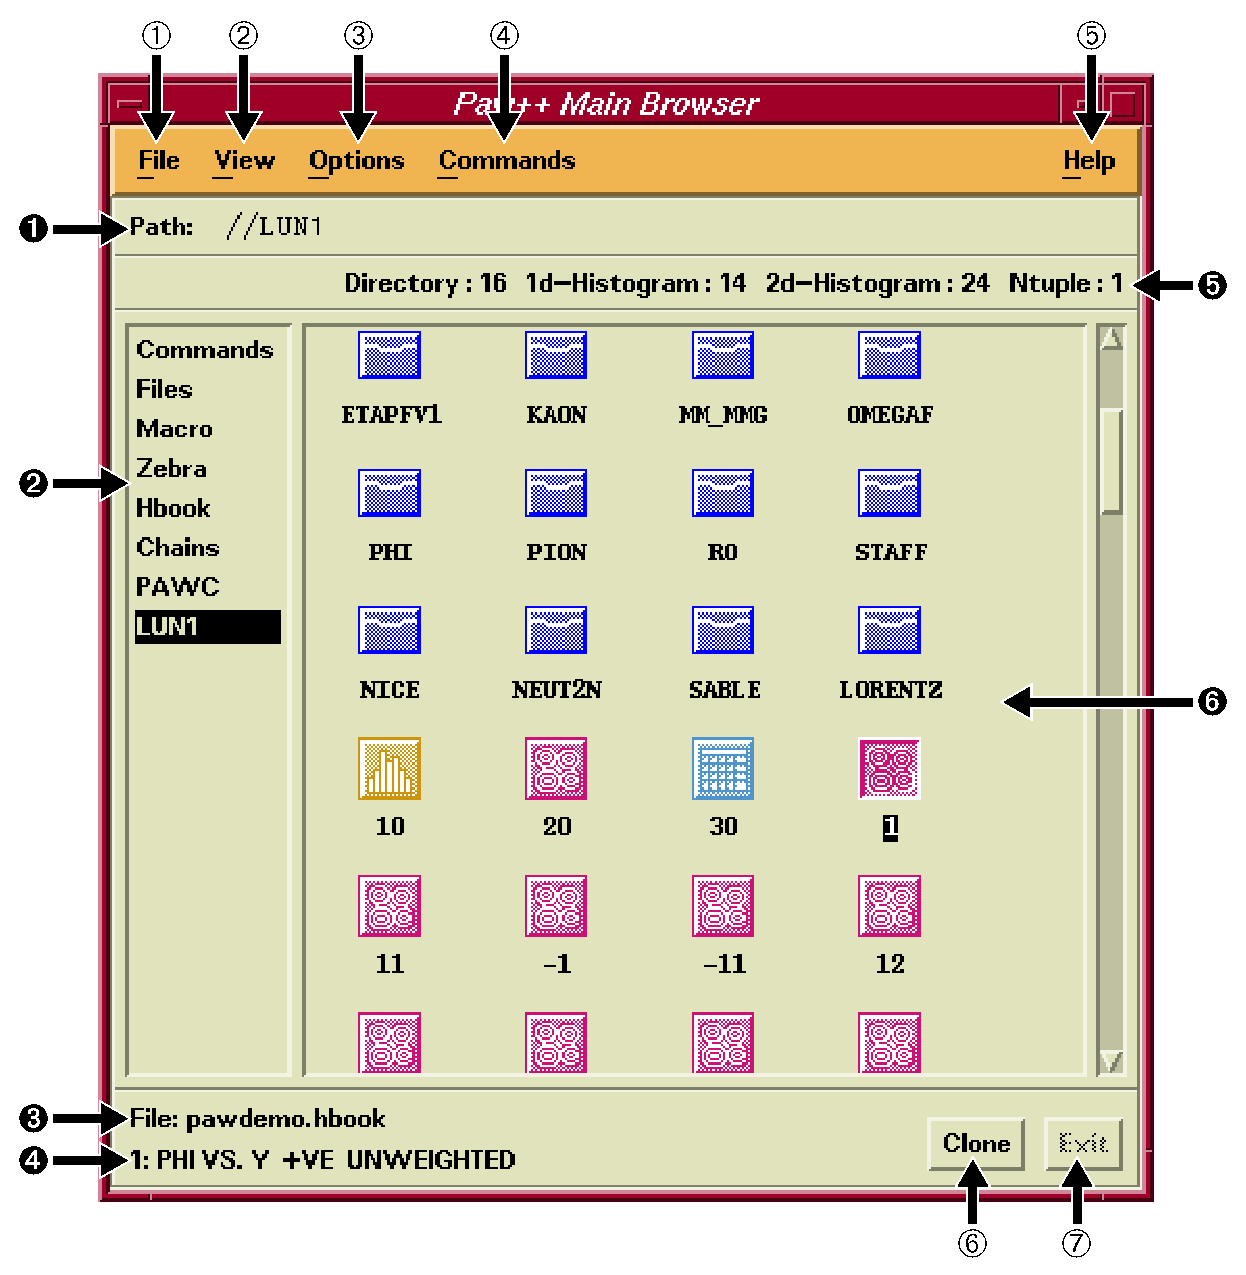
\epsfig{file=browser.eps,height=\textwidth}
\end{sideways}
\caption{\KUIPMotif{} object browser.
\label{fig-motif-browser}}
\end{figure}

\subsection{Browser terminology}

The main part of the browser (figure~\ref{fig-motif-browser})
is taken by the \textem{content window} to display \textem{objects} as 
\textem{icons}.
Each object is identified by its \textem{name} and its type or \textem{class}.
The \Lit{>Class} directive defines new classes and determines the
icons to be used for displaying the objects.

The objects are attached to container objects called \textem{browsables}.
Browsables are identified by a name and a class as well.
The \textem{class window} to the left of the content window displays the
list of browsables known to the browser.
The \Lit{>Browse} directive has to give for each browsable class a 
\textsl{next-object} routine which has to be provided by the application.
The browser calls this routine in order to retrieve the list of
objects which should be displayed in the content window.

A browsable can also contain a tree structure of objects by defining a
special object class for \textem{directories} containing other objects.
The browser keeps track of the current directory path for each
browsable.
The current path for the selected browsable is displayed in the 
\textem{path window} above the class window.
When changing into a subdirectory the new directory path is formed by
concatenating the old path, a ``\Lit{/}'', and the name of the
directory object.
This new directory path is then passed to the \textsl{next-object}
routine in order to retrieve the objects contained in the
subdirectory and to update the content window.

\subsection{The ``next-browsable'' routine}

In frequent cases browsables are stored in external files and a
variable number of them can be connected to the browser.
The \Lit{Browse} directive allows to specify a \textsl{next-browsable}
routine to retrieve the list of currently connected browsables from the
application.

\begin{figure}[tb]
\begin{XMP}
      SUBROUTINE next_browsable(
     +   browsable_name, browsable_class, meta_variables )
      CHARACTER*(*) browsable_name, browsable_class, meta_variables
         ...
      SAVE next_counter

      IF( browsable_name .EQ. ' ' ) THEN
         next_counter = 1
      ELSE
         next_counter = next_counter + 1
      ENDIF

*--- find <next_counter> browsable of requested browsable_class
         ...

      IF( no_more_browsables_left ) THEN
         browsable_name = ' '
      ELSE
         browsable_name = ...
         meta_variables = ...
*--- e.g. 'root=//LUN1 unit=1 file=myfile.hbook'
      ENDIF
      END
\end{XMP}
\caption{Skeleton for a \textsl{next-browsable} routine in Fortran.
\label{fig-next-browsable}}
\end{figure}

The \textsl{next-browsable} routines are iterator functions, i.e.\ they
have to return one browsable at a time.
Figure~\ref{fig-next-browsable} shows the skeleton for a 
\textsl{next-browsable} routine in Fortran.
For each browsable class the browser calls the corresponding routine
in a loop. 
Before the first call \Lit{browsable_name} is set to blank and the
loop continues until the returned \Lit{browsable_name} is blank again.

The second argument \Lit{browsable_class} is set to the name of the
browsable class defined by the \Lit{>Browse} directive.
The same \textsl{next-browsable} routine may be used for several
browsable classes by identifying the currently requested class from
\Lit{browsable_class}. 
It is save to do the class identification only once at the first iteration,
i.e.\ when \Lit{browsable_name} is blank on entry.

If the call to \textsl{next-browsable} returns with a non-blank value in
\Lit{browsable_name} a browsable with the give name is added to the
class window.
The output argument \Lit{meta_variables} should contain a blank
separated list of ``\textsl{var}\texttt{=}\textsl{value}'' \textem{meta-variable}
definitions. 



Browsable classes without a \textsl{next-browsable} routine are called
\textem{single-instance} and are pre-connected to the browser.


\subsection{Action menus}

\if0

of the given class which
should be displayed 
can add to the \Lit{File} menu
in the browser's top menu bar actions
Each browsable class in the class window.
an action menu to operate
on the currently selected browsable.

contained in a
n application-supplied
browsable. 

 and the menus from which an \textem{action} on the selected object
can be chosen. 

 and most of the \Motif{}-specific \CDF{} directives deal with the
customization of the browser.
An application can define in the \CDF{} new types of objects 
(\textem{classes}) to be accessible by the browser.

The selected object (command \Lit{HELP}) is high-lighted and pressing
the right-hand mouse button pops up an \textem{action menu}.
The icons and action menus depend on the object \textem{class} and have
to be defined in the \CDF{}.

The objects are contained in \textem{browsables}
The \textem{class window} to the left of the content window 

The class definition also has to specify a routine which the browser
can call to retrieve the objects contained in the current directory.
This routine has to return the \textem{class name} ``\Lit{Command}'' and
the \textem{object name} ``\Lit{HELP}'' (which must be unique within the
current directory). 
Each item in an action menu allows to specify a \textem{command sequence}
to be executed.
The \textem{meta-variable} ``\Lit{[this]}'' in the command sequence is
replaced by the name of the selected object.

Each object can have two additional attributes: a short and a long
description text.
The meta-variable ``\Lit{[that]}'' refers to the short text and allows
to use it as \textem{object alias}.
The long text ``\Lit{[ ITEM OPTION ]}'' and the name of the selected
object is displayed in the \textem{object description} at the bottom of
the browser. 
The ``\Lit{View}'' pull-down menu allows to choose between different
ways of displaying the objects in the content window:
\begin{UL}
\item Big icons and object name
\item Small icons and object name
\item Object name and short text (no icons)
\item Small icons, object name, short text, and long text
\end{UL}
The vertical scroll bar to the right of the content window allows to
see different sections of the content window.
The total object count ``\Lit{Menu : 2  Command : 12}'' is displayed
in the \textem{summary line} just above the content window.


Directories are a special object class 


\begin{Gray}{i}
>BROWSE  class-name  title-text  next-object  next-browsable
\end{Gray}
The \Lit{>Browse} directive defines a browsable class 
\textsl{class-name}.
\textsl{Title-text} is used for the pop-up menu header in the class
window.
\textsl{Next-object} and \textsl{next-browsable} are the names of routines
which have to be supplied by the application.
\textsl{Next-object} is called by the browser in order to retrieve the
objects contained in a browsable. 
\textsl{Next-browsable} is called to retrieve the list of connected
browsables. 
In simple cases a \textsl{next-browsable} routine need not be defined
(see below).


The \Lit{>Browse} directive is followed by two action lists
separated by a line containing on a ``\Lit{+}'' character in the first
column: 
\begin{XMP}
\textsl{action list for class window}
+
\textsl{action list for {\tt File} menu}
\end{XMP}
The action lists define the menus of possible actions with
each line containing the fields:

\indent\indent\begin{tabular}{cccc}
\textsl{menu-text} &  $[$ \textsl{option-flags} & \textsl{command-sequence}
& \textsl{call-back-routine} $]$
\end{tabular}
\vskip\parskip

The fields are positional separated by blanks.
A field value containing embedded blanks must be enclosed in quotes.
Empty fields have to specified as a single ``\Lit{.}'' character.
Empty fields at the end of a line may be omitted.

\textsl{Menu-text} is the text which will be displayed in the menu.
\textsl{Option-flags} can contain the special characters:
\begin{UL}
\item ``\Lit{/}'' to insert a separator line above the menu item.
\item ``\Lit{!}'' to flag actions which create or delete objects.
This option is required to force updating all browser windows which
could be affected by a change in the object content.
\end{UL}

\textsl{Command-sequence} allows to defines a command string which should be
executed when the corresponding menu item is selected.
The command string can contain several commands separated by
``\Lit{;}''.
The semicolon should be followed by a blank to avoid the exception
rules when ``\Lit{;}'' is not treated as a command separator.
Meta-variables ``\Lit{[}\textsl{var}\Lit{]}'' inside the command string
allow to refer to the selected browsable.
They are replaced by the values defined by the \textsl{next-browsable}
routine (see below for the meta-variables with a predefined meaning).

After replacing the meta-variables the commands are executed as if
they were typed in. 
Command names may be abbreviated but should at least contain a partial
menu path to avoid conflicts if the user defines aliases or changes
the command root with \Lit{SET/ROOT}. 
A command provided with all mandatory arguments is usually executed
immediately. 
The immediate execution can be inhibited by preceding the command name
with a ``\Lit{-}''~character.
As in the case of missing mandatory arguments the ``\Lit{-}'' forces the
display of the corresponding command panel derived from the \CDF{} (see
figure~\ref{fig-motif-panel}). 

\begin{figure}[htb]
\begin{sideways}
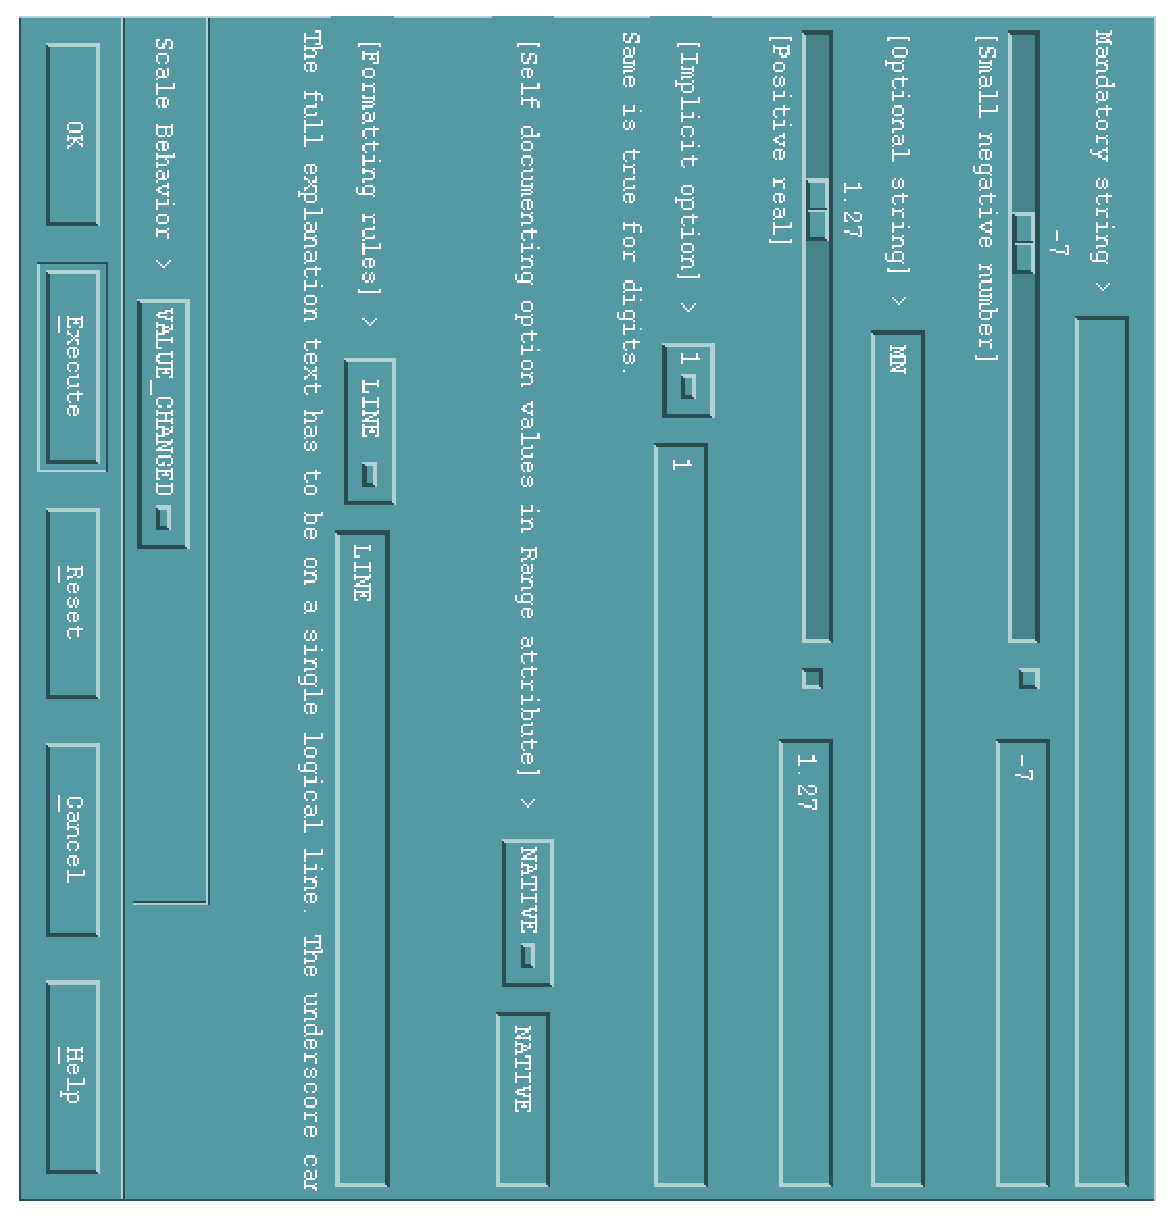
\epsfig{file=xechopanel.eps,height=.47\textwidth}
\end{sideways}
\hspace{\fill}
\begin{sideways}
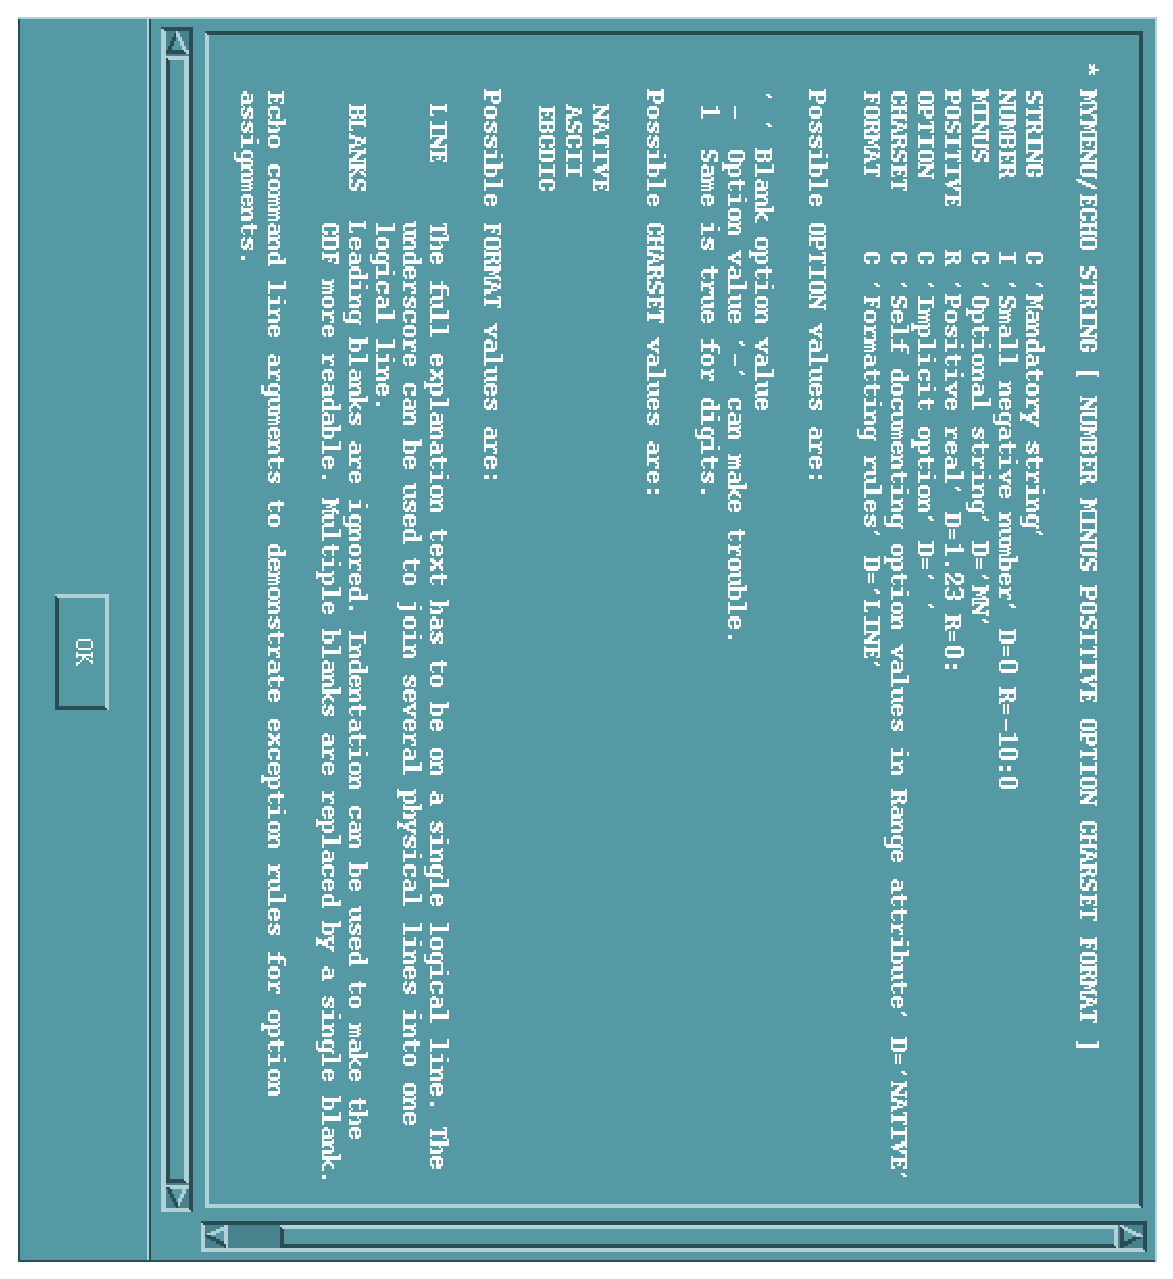
\epsfig{file=xechohelp.eps,height=.49\textwidth}
\end{sideways}
\caption{\Motif{} command panel and help window from \CDF{} example.
\label{fig-motif-panel}}
\end{figure}

The panel allows the user to fill in or change argument values before
executing the command.
The ``\Lit{-}'' should also be used for destructive commands 
(e.g.\ delete object or close file) to allow the user to cancel the execution.
Each panel provides five buttons:
\begin{UL}
\item \Lit{OK} executes the command and destroys the panel.
\item \Lit{Execute} executes the command but keeps the panel for
further command executions.
\item \Lit{Reset} resets all parameters to their default values.
\item \Lit{Cancel} destroys the panel without executing the command.
Further commands in the same \textsl{command-sequence} are ignored.
\item \Lit{Help} displays the help text in a separate window.
\end{UL}
To ensure the sequential execution of a command sequence the \Motif{}
event loop is blocked for all but the last command, i.e.\ 
the user has to press either the \Lit{OK} button or the \Lit{Cancel}
button before the application can continue.

The user can also force the panel display for each command in the
sequence by holding the \Lit{CTRL}-key before popping\footnote{
The \Motif{} implementation of pop-up menus does not allow to sense key
presses during the pop-up display.}
the menu.
The user-forced panel display can be inhibited by preceding the
command name by a ``\Lit{+}''~character.
This should be used in sequences where changing the arguments may
jeopardize the successful execution of subsequent commands, e.g.\ for
a directory change followed by a command using a relative path only.
Obviously the corresponding ``\Lit{+}''~command has to be provided with all
mandatory arguments in order to be executable.

For special applications the action line may also define a 
\textsl{call-back-routine} to be called when the corresponding menu item
is selected. 
(If a \textsl{command-sequence} is defined as well the \textsl{call-back-routine}
is called after executing the commands.)
\textsl{Call-back-routine} may either be the name of a Fortran routine or
the name of C~function followed by ``\Lit{\%C}''.
For a Fortran routine the calling sequence depends on the
action menu for which it is defined (see below).



In addition or as an alternative to a command sequence 

For sequences where subsequent commands depend on that


 of and some arguments may be omitted.

The command definitions explained in the previous section are used by
the \KUIPMotif{} interface to generate command panels where the user can
fill in missing arguments or change default values.
Figure~\ref{fig-motif-panel} shows the panel created automatically
from the \Lit{ECHO} command example.


A minimum set of meta-variables has to be defined by the 
\textsl{next-browsable} routine:
\begin{UL}
\item \Lit{[name]} as the name of the browsable.
\item \Lit{[root]} as the initial setting for \Lit{[path]}.
\item \Lit{[file]} as the text which should be displayed at the bottom
of the browser.
\end{UL}

Note that all fields in an action line are positional 

 to contains a ``\Lit{/}'' character 

The first action list defines the pop-up menu for the browsable selected
in the class window.
The second action list add items to the \Lit{File} pull-down menu.
This allows to define to define the necessary actions to connect
browsables which are stored in external files.

is a browsable class 
\textsl{class-name}.

Figure~\ref{fig-next-object} shows the skeleton for 
\fi

\begin{figure}[htb]
\begin{XMP}
      SUBROUTINE next_object(
     +   browsable_name, browsable_class, current_path,
     +   object_name, object_class, short_text, long_text )
      CHARACTER*(*) browsable_name, ..., long_text
         ...
      SAVE next_counter

      IF( object_name .EQ. ' ' ) THEN
*--- first object is requested
         next_counter = 1

*--- identify from browsable_name, browsable_class
*--- and current_path which objects are requested
            ...
      ELSE
*--- next object is requested
         next_counter = next_counter + 1
      ENDIF

*--- find object with number next_counter
         ...

      IF( no_more_objects_left ) THEN
*--- stop scanning process
         object_name = ' '
      ELSE
*--- mandatory return values
         object_name = ...
         object_class = ...

*--- optional return values
         short_text = ...
         long_text = ...
      ENDIF
      END
\end{XMP}
\caption{Skeleton for the \textsl{next-object} routine.
\label{fig-next-object}}
\end{figure}

\if0
and is followed
by the menu definitions
\begin{XMP}\tt
\textsl{action list for class window} 
+ 
\textsl{action list for File menu}
\end{XMP}

the routine which should be called after decoding the command line in
order to perform the intended operations.

%\end{minipage}


\section{Example of \CDF{} files}

Below we list an example of a \CDF{} (being in fact the first part of the \CDF{} of PAW),
and the corresponding Fortran code generated by the \KUIP{} Compiler.
%
%---------------------------------------------------------------------------
%
\begin{XMPtext}{Example of a \CDF{} file}
>Name HISDEF
 
>Menu HISTOGRAM
>Guidance
Manipulation of histograms, Ntuples.
Interface to the HBOOK package.
 
>Command FILE
>Parameters
LUN 'Logical unit number' I R=1:128
FNAME 'File name' C
+
LRECL 'Record length in words' I D=1024
CHOPT 'CHOPT' C D=' ' R=' ,N,U'
>Guidance
Open an HBOOK direct access file.
 For CHOPT=' ', existing file opened (read only).
 For CHOPT='N', a new file is opened.
 For CHOPT='U', existing file opened to be modified.
>Action PAHIST
 
>Command LIST
>Parameters
+
CHOPT 'Options' C D=' ' R=' ,I'
>Guidance
List the histograms in the current directory (memory or disk).
Histograms are all HBOOK objects including Ntuples.
If CHOPT='I' a verbose format is used (batch: HINDEX).
>Action PAHIST
\end{XMPtext}
\newpage
\begin{XMPtext}{Fortran code generated from the \CDF{}}
*     -------------------
      SUBROUTINE HISDEF
*     -------------------
      INTEGER MGUIDL
      PARAMETER (MGUIDL=199)
      CHARACTER*80 GUID
      COMMON /KCGUID/ GUID(MGUIDL)
      EXTERNAL PAHIST
      EXTERNAL HISDEH
 
      CALL KUNWG(  -1)
      CALL KUCMD(' ','HISTOGRAM','C')
      CALL KUACG('HISTOGRAM',HISDEH)
      CALL KUCMD('HISTOGRAM',' ','SW')
 
      CALL KUNWG(  -2)
      CALL KUCMD(' ','FILE','C ')
      CALL KUNDPV(  1,  1,  1,  0,  1)
      CALL KUPAR('FILE','LUN','Logical unit number','I ','S')
      CALL KUPVAL('FILE','LUN',1,0.,' ','L')
      CALL KUPVAL('FILE','LUN',128,0.,' ','H')
      CALL KUNDPV( 1, 1, 1, 0,  1)
      CALL KUPAR('FILE','FNAME','File name','C ','S')
      CALL KUNDPV(  1,  1,  1,  0,  1)
      CALL KUPAR('FILE','LRECL','Record length in words','IO','S')
      CALL KUPVAL('FILE','LRECL',1024,0.,' ','D')
      CALL KUNDPV( 1, 1, 1, 1,  2)
      CALL KUPAR('FILE','CHOPT','CHOPT','CO','S')
      CALL KUPVAL('FILE','CHOPT',0,0.,' ,N,U','V')
      CALL KUPVAL('FILE','CHOPT',0,0.,' ','D')
      CALL KUACG('FILE',HISDEH)
      CALL KUACT('FILE',PAHIST)
 
      CALL KUNWG(  -3)
      CALL KUCMD(' ','LIST','C ')
      CALL KUNDPV( 1, 1, 1, 1,  1)
      CALL KUPAR('LIST','CHOPT','Options','CO','S')
      CALL KUPVAL('LIST','CHOPT',0,0.,' ,I','V')
      CALL KUPVAL('LIST','CHOPT',0,0.,' ','D')
      CALL KUACG('LIST',HISDEH)
      CALL KUACT('LIST',PAHIST)
 
      CALL KUNWG(   0)
      CALL KUNDPV(   1,   1,   1,   0,   1)
      CALL KUCMD(' ',' ','E')
      CALL KUCMD('/',' ','SW')
      END
*     -------------------
      SUBROUTINE HISDEH
*     -------------------
      INTEGER MGUIDL
      PARAMETER (MGUIDL=199)
      CHARACTER*80 GUID
      COMMON /KCGUID/ GUID(MGUIDL)
      COMMON /KCGUIL/ NGLN
*
      GOTO( 1, 2, 3),NGLN
*
* HISTOGRAM
*
    1 CONTINUE
      GUID( 1)='Manipulation of histograms, Ntuples. '
      GUID( 2)='Interface to the HBOOK package. '
      NGLN=  2
      GOTO 9999
*
* HISTOGRAM/FILE
*
    2 CONTINUE
      GUID( 1)='Open an HBOOK direct access file. '
      GUID( 2)=' For CHOPT='' '', existing file opened (read only).'
      GUID( 3)=' For CHOPT=''N'', a new file is opened. '
      GUID( 4)=' For CHOPT=''U'', existing file opened to be modified.'
      NGLN=  4
      GOTO 9999
*
* HISTOGRAM/LIST
*
    3 CONTINUE
      GUID( 1)='List the histograms in the current directory (memory or
     +disk). '
      GUID( 2)='Histograms are all HBOOK objects including Ntuples. '
      GUID( 3)='If CHOPT=''I'' a verbose format is used (batch: HINDEX).
     + '
      NGLN=  3
      GOTO 9999
9999  RETURN
      END
\end{XMPtext}
%
%---------------------------------------------------------------------------
%
\fi
\fi

\section{Various Hints specific to \KUIPMotif{}}
 
\subsection{ C-callable Interface to the Panel Interface}
 
A C-callable interface for the complete \Cind{PANEL} interface (panels and
palettes) built-in inside \KUIPMotif{} (see \ref{ref:repanel})
is accessible to the application programmer. This allows him
to set up some predefined panels without having to transport
independent macro files together with the application executable,
and having to refer them in the logon macro file.
This is the case, for example,  of the graphical editor ``Ged'' which makes
an intensive use of graphical and alphanumerics ``programmer-defined''
panels.
 
The C callable entries are:

\begin{Gray}{l}
void km_panel_reset()
\end{Gray}
Reset panel in memory (<>~``\Lit{panel 0 r}'').

\begin{Gray}{l}
void km_panel_key( int row, int col,  char *command, 
                   char *alias_label, char *pixmap )
\end{Gray}
\Pdesc\begin{DLtt}{\mbox{\hspace{7em}}}
\item[row] row number
\item[col] column number
\item[command]  command (or list of commands) to be executed
\condbreak{2\baselineskip}
\item[alias_label] alias name for command (or NULL)
\item[pixmap] pixmap representation for button label (or NULL)
\end{DLtt}
Define key (<>~``\Lit{panel x.y ...}'').

\begin{Gray}{l}
void km_panel_display( char *title, char *geometry )
\end{Gray}
\Pdesc\begin{DLtt}{\mbox{\hspace{7em}}}
\item[title] panel title
\item[geometry] panel geometry
  (\textsl{w}\texttt{x}\textsl{h}\texttt{+}\textsl{x}\texttt{+}\textsl{y}) 
\end{DLtt}
Display panel (<>~``\Lit{panel 0 d ...}'').

\begin{Gray}{l}
void km_panel_close( char *title )
\end{Gray}
\Pdesc\begin{DLtt}{\mbox{\hspace{7em}}}
\item[title] panel title
\end{DLtt}
Close panel with given title (<>~``\Lit{panel 0 c ...}'').

\begin{Gray}{l}
void km_icon( char *icon, char *fname )
\end{Gray}
\Pdesc\begin{DLtt}{\mbox{\hspace{7em}}}
\item[icon] icon name
\item[fname] filename (output of the X11 utility bitmaps).
\end{DLtt}
Store icon data from a bitmap file (<>~``\Lit{motif/icon ...}'').

\begin{Gray}{l}
void km_palette( char *title, char *geometry )
\end{Gray}
\Pdesc\begin{DLtt}{\mbox{\hspace{7em}}}
\item[title] palette title
\item[geometry] palette geometry (wxh+x+y)
\end{DLtt}
Open or close a ``multi-panel'' (palette) widget
(<>~``\Lit{motif/multi_panel ...}'').
 
The routine (written by the application programmer) which contains
all the panels definition has to be called via the ``Motif\_customize''
mechanism (described is section \ref{ref:rehooks}) in the so-called
``widget-routine'' (its has to be called before entering the Motif
main loop, but after initialization).
 
E.g.:
\begin{XMP}
>Motif\_customize . init_top_level_window%C
\end{XMP}
 
The following is an illustration of how to use these routines. On
the left side you have the KUIP macro file for a panel definition, and
on the right side you have the equivalent coded in~C. The C~routine
\texttt{my_panel_definition} is automatically called by KUIP,
just after the creation of the \EW{} (kxterm), thanks
to the \CDF{} directive ''Motif\_customize''.
(See the code of the ``widget-routine'' \texttt{init_top_level_window} at the end
of the ``C~Interface'' side).
\vfill 
\begin{XMP}
**************           |     /***************/
* KUIP Macro *           |     /* C Interface */
**************           |     /***************/
 
                         |     #include <X11/Intrinsic.h>

                         |     extern void km_icon();
                         |     extern void km_panel_reset();
                         |     extern void km_panel_display();
                         |     extern void km_panel_key();

                         |     my_panel_definition()
                         |     \{
*
* Icon bitmaps
*
/motif/icon m1 mk1.bm    |       km_icon ("m1", "/user/cremel/ktest/mk1.bm");
/motif/icon m2 mk2.bm    |       km_icon ("m2", "/user/cremel/ktest/mk2.bm");
/motif/icon m3 mk3.bm    |       km_icon ("m3", "/user/cremel/ktest/mk3.bm");
/motif/icon m4 mk4.bm    |       km_icon ("m4", "/user/cremel/ktest/mk4.bm");
/motif/icon m5 mk5.bm    |       km_icon ("m5", "/user/cremel/ktest/mk5.bm");
 
*
* Panel keys definition
*
panel 0                  |       km_panel_reset();
panel 2.01 null          |       km_panel_key (2, 1, "null", NULL, NULL);
panel 2.02 tex_1         |       km_panel_key (2, 2, "tex_1", NULL, NULL);
panel 3.01 '/example/general kuip.tex tex 1' 'tex_1' m1
                         |       km_panel_key (3, 1, ...
                           ..."/example/general kuip.tex tex 1", "tex_1", "m1");
panel 3.02 '/example/general kuip.tex tex 2' 'tex_2' m2
                         |       km_panel_key (3, 2, ...
                           ..."example/general kuip.tex tex 2", "tex_2", "m2");
panel 3.03 '/example/general kuip.tex tex 3' . m3
                         |       km_panel_key (3, 3, ...
                           ..."example/general kuip.tex tex 3", NULL, "m3");
panel 3.04 '/example/general kuip.tex tex 4' . m4
                         |       km_panel_key (3, 4, ...
                           ..."example/general kuip.tex tex 4", NULL, "m4");
panel 4.01 ' ' . m5      |       km_panel_key (4, 1, " ", NULL, "m5");
panel 4.02 'tex_5' . m5  |       km_panel_key (4, 2, "tex_5", NULL, "m5");
panel 5.01 '/example/general kuip.tex tex 6' . m6
                         |       km_panel_key (5, 1, ...
                           ..."example/general kuip.tex tex 6", NULL, "m6");\condbreak{3\baselineskip}
panel 5.02 '/example/general kuip.tex tex 6' . big_menu
                         |       km_panel_key (5, 2, ...
                           ..."example/general kuip.tex tex 6",NULL,"big_menu");
panel 6.01 '/example/general kuip.tex tex 7' 'tex_7'
                         |       km_panel_key (6, 1, ...
                           ..."example/general kuip.tex tex 7", "tex_7",NULL);
panel 6.02 '/example/general kuip.tex tex 7' 'tex_7' m1
                         |       km_panel_key (6, 2, ...
                           ..."example/general kuip.tex tex 7", "tex_7", "m1");
 
* Open a palette (multi_panel)
multi_panel 'Marker Palette' '300x1000-0+0'
                         |       km_palette ("Marker Palette", "300x1000-0+0");
 
* Display panel(s)
panel 0 d 'Marker Types' 300x300+500+500
                         |       km_panel_display ("Marker Types", ...
                           ..."300x300+500+500");
 
* Close current palette
multi_panel 'end'        |       km_palette ("end", NULL);
                         |     \}
 
                         |     void init_top_level_window(name, top)
                         |         char *name;
                         |         Widget top;
                         |     \{
                         |       if (strcmp(name,"kxterm") == 0) \{
                         |         my_panel_definition();
                         |       \}
                         |     \}
\end{XMP}
 
 
\subsection{User-Defined Single Selection Lists}
 
It is possible in \KUIPMotif{} to set up a command which displays a
list of various items or choices (instead of the usual command
argument panel with the list of arguments to be filled).
This is,
for instance, the behavior of the command ``HELP'' in \KUIPMotif{}:
if you type ``help'' without any argument a selection box with all
possible help menus or items is displayed and the user can select
one (or just cancel the execution) and get the appropriate help information.
 
Note that the argument type ``list'' does not exist in the basic
\KUIP{} and we thought that the most frequent case is probably
the one mentioned above, i.e.\ a command which displays a predefined list
(or set up at run time). In such a case one should get access
to the ``Selection Box'' widget in a so-called Motif interface.
 
To implement such a command the application-programmer has to define
in the CDF (with the other application defined commands) a new command
without any argument and the action routine written in~C. 
E.g.:
\begin{XMP}\condbreak{2\baselineskip}
>Menu EXAMPLE
...
>Command LIST
>Guidance
This is just an example of a command which
displays a list of items.
(See action routine ktactc.c)
>Action ktactc%C
\end{XMP}
We provide in \KUIPMotif{} two user-callable C~routines (\texttt{km_list_data}
and \texttt{km_show_list} which make the implementation of this ``list display''
quite easy (no Motif code is involved). These routines have to be called
directly in the code of the action routine. The part which concerns the
filling of the list and the action to execute after a selection has been
done (<OK> button pressed) is (obviously) application dependent.
 
Description of these two user-callable C~routines:

\begin{Gray}{i}
void km_list_data( char *list_label, char *selection_label,
                   char *help_text,  int call_back(char* selection) )
\end{Gray}
\Pdesc\begin{DLtt}{\mbox{\hspace{7em}}}
\item[list_label]  label (prompt) written at the beginning of the list
\item[selection_label]  label (prompt) written before the selection
\item[help_text]  help message accessed through help button
\item[call_back]  user defined routine called when the OK is pressed.
  The value selected by the user is passed as argument when the
  routine is called.
\end{DLtt}
Fill the application data for a user-defined list.
All parameters are application dependent.

 
\begin{Gray}{i}
void km_show_list( char **items )
\end{Gray}
\Pdesc\begin{DLtt}{\mbox{\hspace{7em}}}
\item[items]  list of items (choices) in the list.
\end{DLtt}
Displays the list.
 
The following is a skeleton (some parts have to be filled according to
the application) for the application routine \texttt{ktactc.c} for the
new command ``LIST'' described above:
\begin{XMP}
/* Listing of file ktactc.c */
 
#ifndef NULL
#define NULL 0
#endif
 
/***************************************************************/
/*                                                             */\condbreak{3\baselineskip}
/* Action routine for command "/EXAMPLE/LIST"                  */
/* (Example of how to display a "user defined" list            */
/*  with KUIP/Motif).                                          */
/*                                                             */
/***************************************************************/
 
ktactc()
\{
  int ktactc_OK ();
  int i;
 
  static char *help_text = "You can write there \bs{}n\bs{}
some help text for \bs{}"My List\bs{}" ...";
 
  /* List of all items (can be filled dynamically) */
  char **list_item = (char **) malloc ( sizeof (char *) );
 
  /* Fill list data: */
  km_list_data
     ("My List Label", "My List Selection", help_text, ktactc_OK);
 
  /* Fill list of items (with 10 arbitrary values) ...
   * ... N.B. Write your application defined code here ... i
   */
  for (i = 0; i < 10; i++) \{
       list_item = (char **) realloc( (char*)list_item,
                                        (i+1) * sizeof (char *) );
       list_item[i] = (char *) malloc (10);
       sprintf (list_item[i], "item %d", i+1);
  \}
  list_item = (char **) realloc( (char*)list_item, (i+1) * sizeof (char *) );
  list_item[i] = NULL;
 
  /*
   * Display list and wait for user action ...
   * ... N.B. If user action is "OK" you go into
   * the "OK call-back" defined by km_list_data (ktactc_OK)
   * - See example for code of ktactc_OK above _
   */
  km_show_list (list_item);
 
  for (i = 0; i < 10; i++) free (list_item[i]);
  free (list_item);
\}
\vfill 
/*
 * Routine name (ktactc_OK) is defined by KM_list_data.
 * This routine is automatically called when pressing the "OK" button.
 *      char *val (input) : value issued from the user selection
 *
 */
int ktactc_OK (val)
    char *val;
\{
    printf ("*** display_list_OK : (ktactc_OK)\bs{}n");
    printf ("    value selected in the list %s.\bs{}n", val);
 
    return 0;
\}
\end{XMP}
 
Picture \ref{ref:FIGPKMF192} shows the output from
\KUIPMotif{} when executing the command ``/EXAMPLE/LIST'' described above.

\begin{figure}[htb]
\hfill
\begin{PICTf}[.4]{pkmf192}
\end{PICTf}
\hfill
\caption{User-defined List in a Command}
\label{ref:FIGPKMF192}
\end{figure}
 
\subsection{User-Defined File Selection Boxes}
 
It is also possible with \KUIPMotif{} to set up a command which displays a
"FileSelectionBox" (conform to the Motif terminology) containing:
\begin{UL}
\item
a ``Filter'' entry to select only files with a certain pattern,
\item
a ``Directories'' entry to select the directory applied to the ``Filter''
(this can also be done by editing the ``Filter'' entry manually),
\item
a ``Files'' entry, with the list of all files corresponding to the
``Filter'' selected.
\end{UL}
This is a very convenient way to select a file name, and being able to
scan the directory tree.
 
To implement such a command the application-programmer has to define
in the CDF (with the other application defined commands) a new command
without any argument and the action routine written in C. E.g.:
\begin{XMP}
>Menu EXAMPLE
...
>Command SELECT_FILE
>Guidance
This is just an example of a command which
displays a file list selection box.
(See action routine ktactcf.c)
>Action ktactcf%C
\end{XMP}
We provide the user-callable a C~routine (\Lit{km_show_filSel})
which makes the implementation of this ``FileSelectionBox''
quite easy (no Motif code is involved). It has to be called
directly in the code of the action routine. The part which concerns the
data setting and the action to execute after a selection has been
done (<OK> button pressed) is (obviously) application dependent.
 
N.B. You get automatically to this "FileSelectionBox" by defining a
parameter type ``FILE'' (extension to the type ``\Lit{C}'' (character) in the
\CDF{}). But this C user-callable routine
gives the application programmer the
possibility to define commands that directly display a
"FileSelectionBox" (without producing the usual ``Command Argument Panel'')
and also to fill the data (filter, default value) at run time.
 
Description:
\begin{Gray}{i}
void km_show_filSel( char *title, char *dir, char *def, char *help,
                     int call_back(char* selection) )
\end{Gray}
All parameters (input) in this routine are application dependent.
\Pdesc\begin{DLtt}{\mbox{\hspace{7em}}}
\item[title] title of the FileSelectionBox
\item[dir] directory (for filter)
\item[def] default file name
\item[help] help text (accessed through help button)
\item[call_back]  user defined routine called when the ``OK'' button
  is pressed. 
  The value selected by the user is passed as argument when the
  routine is called.
\end{DLtt}
 
The following is a skeleton (some parts have to be filled according to
the application) for the application routine \texttt{ktactcf} for the
new command \Cind{SELECT_FILE} described above:
\begin{XMP}
/* ktactcf.c */
 
#include <stdio.h>

extern void km_show_filSel( char *title, char *dir, char *def, char *help,
                            int callback(char* selection) );


/*
 * This routine is automatically called when pressing the "OK" button.
 *      char *val (input) : value issued from the user selection
 */
int ktactcf_OK( char *val )
\{
    printf( "*** fileSelection OK : (ktactcf_OK)\bs{}n" );
    printf( "    File selected is %s.\bs{}n", val );\condbreak{2\baselineskip}
    return 0;
\}
 

/*
 * Action routine for command "SELECT_FILE".
 * (Example of how to display a "user defined" file selection
 *  box with KUIP/Motif).
 */
int ktactcf()
\{
\condbreak{2\baselineskip}
  static char *help_text = "You can write there \bs{}n\bs{}
some help text for \bs{}"My FileSelectionBox\bs{}" ...";
 
    km_show_filSel( "My FileSelectionBox",
                    "/user/cremel/pdemo/*.dat", "hrztest.dat",
                    help_text, ktactcf_OK );
    return 0;
\}
\end{XMP}
 
Picture \ref{ref:FIGPKMF193} shows the output from
\KUIPMotif{} when executing the command \Cind{SELECT_FILE} described
above.

\begin{figure}[htb]
\hfill
\begin{PICTf}[.4]{pkmf193}
\end{PICTf}
\hfill
\caption{User-defined File Selection Box in a Command}
\label{ref:FIGPKMF193}
\end{figure}
 
 
 
\section{Some Examples to Start With}

\subsection{Example 1: Basic Example (No Graphics)}
\label{ref:reexnogr}

This first example is a very simple one in order to show 
\begin{OL}
\item how the different types of parameters handled by \KUIP{} are interpreted 
and visualized in the \Motif{} interface (\CAP{}).
\item what you automatically get with \KUIPMotif{}.
\end{OL}

\subsubsection{The \CAP{} for a Very General Command}

The following \CDF{} defines a new menu ``Example'' and a new command
''General'' with 6 input parameters. The first 2 parameters are mandatory 
and the others are optional.

The action routine to be called at command execution is named KTACT.

\condbreak{3cm}
\begin{XMPt} {Example 1 --- \CDF{} (Command Definition File) ---
ktcdf.cdf}
>Name KTDEF

>Menu Example

>Command General
>Parameters
FILE 'File name' C D='kuip.tex'
OPTION 'Text formatting system' C D='TEX'
-      plain text : plain text format
-LATEX LaTeX format (encapsulated)
-TEX   LaTeX format (without header)
+
LINE 'Number of lines' I D=10
HEIGHT 'Page height (cm)' R D=28.5
LENGTH 'Length of space between sections (cm)' R D=2.5 R=-2.:5.0
PAGE  'Page number' I D=1 R=1:99
>Guidance
This is just an example of a command with different parameter
types.
>Action KTACT
\end{XMPt}

The \CAP{} which is automatically generated by \KUIPMotif{} for this
very general command  ``/EXAMPLE/GENERAL'' is show in
figure~\ref{ref:FIGPKEX1}.

\begin{figure}[tb]
\PICT{pkex1}
\vspace{-1\baselineskip}
\caption{The \CAP{} for command \protect\Cind{EXAMPLE/GENERAL} (Example 1)}
\label{ref:FIGPKEX1}
\end{figure}

\begin{EnumZB}
\item  Parameter 1 (FILE): string input for 'File name' (default is 
'kuip.tex').  This is represented by a ``Text'' widget.
\item  Parameter 2 (OPTION): string input for 'Text formatting system' with
a predefined range of possible values. This is represented by an ``Option 
Menu'' widget + access to a ``List'' widget with the complete description
of the possible options + string input (where the user can write any value
he wants). The default value is 'TEX' and possible values are '~', 'LATEX' 
and 'TEX'.
\item  Parameter 3 (LINE): integer value for the 'Number of lines'. 
This is represented by a ``Text'' widget but an integer value is required 
(default is 10).
\item  Parameter 4: real value for the 'Page height (cm)'. 
This is represented by a ``Text'' widget but a real value is required 
(default is 28.5).
\item  Parameter 5 (LENGTH): real value for the 'Length of space
between sections (cm)'. Possible values have to be within the range
[-2.0...5.0]. This is represented by a ``Scale'' widget (for reals) + 
string input (where the user can write any value he wants). The default value 
is 2.5.
\item  Parameter 6 (PAGE): integer scale for the 'Page number' within the range 
[1...99]. This is represented by a ``Scale'' widget (for integers) +
string input (where the user can write any value he wants). The default value
is 1.
\item This is an option menu which gives the user the possibility to change
the behavior for scales (when real or integer ranges of values are given
for parameters). By default the scale behavior is set to ``VALUE\_CHANGED''
but it can be set to ``DRAG'' which means that the value of the parameter
corresponding to the scale is modified as soon as the user ``drag'' the
scale (and not only when releasing the mouse button on a certain value). 
When the little toggle button next to the scale is highlighted
the command execution is effective as soon as the scale is modified 
without the user has to press the ``OK'' or ``Execute'' button and
whatever the scale behavior setting is (``VALUE\_CHANGED'' or ''DRAG''). 
This allows the user to see dynamically the effect of some parameters
setting: e.g.\ in \PAW++{} for the command ``HISTOGRAM/OPERATIONS/SMOOTH'' 
one can see dynamically the changes in the smoothing algorithm according 
to the value of the ``sensitivity'' or the ``smoothing'' parameters.
\end{EnumZB}

N.B: For parameters 2, 5, and 6 the user has several possibilities
to set the value: option menu, list or scale selection,
or directly string input. In any case it is the value which is written into 
the small text area for string input that is taken for the command execution.
(The option menu, list and scale selection modify automatically the content of 
this text area).

\begin{figure}[htb]\centering
\vspace{-1\baselineskip}
\PICT{pkex2}
\vspace{-2\baselineskip}
\begin{EnumZB}
\item The \EW{} with its menu-bar, the \TP{} and the \INP{} (where users
can type commands).
\item The \MB{}  with its menu-bar, and the predefined \KUIP{} browsables for
the ``Commands'', ``Files'' and ``Macro''.
\item Pulldown menu access to all the commands defined by \KUIP{} and the 
application.
\item The possibility to build panels of commands.
\vspace{-1\baselineskip}
\end{EnumZB}
\caption{What Do You Get? (Example 1)}
\label{ref:FIGPKEX2}
\end{figure}

\subsubsection{Building the Example: What Do you Get?}

The \CDF{} file has to be compiled by the \KUIPC{} compiler into Fortran 
or C~code (according to the file type extension ``\Lit{.f}'' or
``\Lit{.c}'' given to  
the output file). 
With \KUIPMotif{} we require the generation of C~code,
as all the \CDF{} extension specific to \Motif{} (section \ref{ref:recdf})
are only interpreted in the C~output mode of \KUIPC{}. 
The command to be given on any system is
\begin{XMP}
kuipc ktcdf.cdf ktcdf.c
\end{XMP}
which will generate the file \Lit{ktcdf.c}
(to be compiled by the C~compiler)
from the input file \Lit{ktcdf.cdf}.

The following is the application main program in Fortran:

\begin{XMPt} {Example 1 - Main Program - ``ktest\_main.f''}
      PROGRAM KTEST
*
* Basic KUIP Application with MOTIF / NOT linked to HIGZ
*
      COMMON/PAWC/PAW(500000)
*
* Initialize PAW
*
      CALL MZEBRA(-3)
      CALL MZPAW(500000,' ')
*
* Initialize KUIP with NWORDS words as minimum division size
*
      NWORDS=20000
      CALL KUINIT(NWORDS)
*
* Create user command structure from definition file
*
      CALL VECDEF
      CALL KTDEF          ! Command(s) definition part
*                         ! (code generated from the CDF compilation)
*
* Gives access to KUIP browsers for commands, files and macros
*
      CALL KUIDFM
*
* Execute some KUIP Initialization Commands
*
      CALL KUEXEC('PROMPT ''KTEST >''')
      CALL KUEXEC('LAST 0')
*
* Give control to MOTIF
*
      CALL KUWHAM ('Ktest')
*  
      END
\end{XMPt}

We have set the class name of this basic example to ``\Lit{Ktest}'' 
(\Lit{CALL KUWHAM('Ktest')}): this means that the X~resources for the application 
have to be referred with :
\\*[1mm]\mbox{\quad {\Lit{Ktest*}\textsl{<resource\_name>}\Lit{:} \textsl{<resource\_value>} }}

In the action routine (\Cind{KTACT}), coded in Fortran,  we just retrieve and
print the value of all parameters:

\begin{XMPt} {Example 1 - Action Routine KTACT - (``ktact.f'')}
      SUBROUTINE KTACT
*
      CHARACTER*32 CHPATH, CVAL, CHOPT

      DATA LUN/93/
*
* Retrieve command name and number of parameters
*
      CALL KUPATL (CHPATH,NPAR)
*
      IF (CHPATH.EQ.'GENERAL') THEN
*
* Retrieve parameter values
*
           CALL KUGETC (CVAL, IL1)
           CALL KUGETC (CHOPT, IL2)
           CALL KUGETI (ILINE)
           CALL KUGETR (RHEIGHT)
           CALL KUGETR (RLENGTH)
           CALL KUGETI (NBP)
           print *, '===> Command GENERAL:'
           print *, '     File : ', CVAL(1:IL1)
           print *, '     Option : ', CHOPT(1:IL2)
           print *, '     Number of lines: ',ILINE
           print *, '     Page height: ', RHEIGHT
           print *, '     Length of space between sections:', RLENGTH
           print *, '     Page number: ', NBP
      ENDIF
*
 99   RETURN
      END
\end{XMPt}

The link command for \Lit{ktest} is:
\begin{XMP}
f77 -o ktest ktest_main.f ktcdf.c ktact.f `cernlib -G Motif`
\end{XMP}
Fig.~\ref{ref:FIGPKEX2} back on page~\pageref{ref:FIGPKEX2} shows what you
get for this very basic example.

\subsection{Example 2: Application with a Graphical Window Managed by HIGZ}
\label{ref:reexgr}

This second example shows how to build an application which opens a graphical 
window managed by HIGZ and how it is possible to obtain ``direct object
manipulation'' in this graphical window by defining  some specific ``classes''
of objects inside the \CDF{}.

The \CDF{} is divided into 2 parts:
\begin{UL}
\item[1.] {\tt >Name KTDEF} \hfill\break 
it contains the definition for a new menu ``Graphics'' with one command
``Frame\_box'' to draw a frame box with axis. \hfill\break
The action routine to be called at command execution is named KTACTG.
\item[2.] {\tt >Name KTDEFMG} \hfill\break
it contains specific definition for the \KUIPMotif{} interface:
\begin{UL}
\item The directive ``{\tt >Graphics}'' is mandatory for an 
application which requires one (or more) 
graphical window(s) managed by HIGZ.
\item 3 classes of object are defined (``win'', ``x-axis'' and ``y-axis'')
with their specific menu of actions.  These menus apply to objects which 
are identified in the HIGZ graphics window (2nd set of menu separated by a
blank line starting with ``+''). (See section \ref{ref:recdfacm} for more
details).
\end{UL}
\end{UL}

\begin{XMPt} {Example 2 --- \CDF{} (Command Definition File) ---
ktcdfg.cdf}
>Name KTDEF

>Menu Graphics

>Command FRAME_BOX
>Parameters
+
XMIN  'Low range in X'  R D=0. R=0:1000
XMAX  'High range in X' R D=100. R=0:1000
YMIN  'Low range in Y'  R D=0. R=0:1000
YMAX  'High range in Y' R D=100. R=0:1000
CHOPT 'Options'         C D=' '
-  frame box : Draw a frame box only
-S scale : Redefine the scale for the current zone
-A NO axis : Axis labels and tick marks are not drawn
-B NO Box : The box is not drawn
>Guidance
Draw a frame box.
If XMIN, XMAX, etc.\ are given, draw a frame box
with the window coordinates set to XMIN, XMAX, YMIN, YMAX. Axis
labels and tick marks are drawn by default.
>Action KTACTG

>Name KTDEFMG

>Graphics

>Class win 'Graphics Window'
+
 Plot                            . 'Picture/Plot'
'/Do PostScript...'              . '-Picture/Print test.ps'
'Do Encapsulated PostScript...'  . '-Picture/Print test.eps'
'Do LaTex...'                    . '-Picture/Print test.tex'
'Print'                          . 'Picture/Print'
'/Open New Window'               . 'Work [this] OA'
'Close Window'                   . 'Work [this] C'
'Activate Window'                . 'Work [this] A'
'Deactivate Window'              . 'Work [this] D'

>Class x-axis 'X Axis'
+
'Logarithmic'    . 'OPTION LOGX'
'Linear'         . 'OPTION LINX'
'Color'          . 'SET XCOL'
'Character Font' . 'SET VFON'
\condbreak{3\baselineskip}
>Class y-axis 'Y Axis'
+
'Logarithmic'    . 'OPTION LOGX'
'Linear'         . 'OPTION LINX'
'Color'          . 'SET XCOL'
'Character Font' . 'SET VFON'
\end{XMPt}

N.B. The object class ``win'' is predefined inside \HIGZ{} itself (see the
\HIGZ{} documentation for routine \IGOBJ{}) in order to refer the graphics 
window when no other object with a higher level has been identified.
This is a very convenient  facility for defining a popup menu associated
to a graphics window managed by HIGZ: the only thing to do is to describe 
this menu of actions in the \CDF{} following the directive 
{\tt ``>Class win ...''} (as done in our example).

The following is the application main program in Fortran:

\begin{XMPt} {Example 2 - Main Program - ``ktestg\_main.f''}
      PROGRAM KTEST
*
* Basic KUIP/Motif Application with HIGZ graphics window
*
      PARAMETER (NWHIGZ=10000)
      COMMON/PAWC/PAW(500000)
*
      EXTERNAL      IGTERM
*
* Initialize PAW
*
      CALL MZEBRA(-3)
      CALL MZPAW(500000,' ')
*
* Initialize KUIP with NWORDS words as minimum division size
*
      NWORDS=20000
      CALL KUINIT(NWORDS)
*
* Create user command structure from definition file (CDF)
*
      CALL VECDEF
      CALL KTDEF          ! Command(s) definition part
*                         ! (code generated from the CDF compilation)
*
* Gives access to KUIP browsers for commands, files and macros
*
      CALL KUIDFM
*
* Special KUIP initialization for using Motif with HIGZ
*
      CALL KTDEFMG        ! Graphics and class(es) definition
*                         ! (code generated from the CDF compilation)
      CALL KUINIM('Ktestg')
*
* Initialize HIGZ
*
      CALL IGINIT(NWHIGZ)
      CALL KUGRFL(IGTERM)   ! flush the graphics output after each command
*
* Initialize HPLOT
*
      IWK=999
      CALL HPLINT(IWK)
      CALL IGSA(0)
*
* Execute some KUIP Initialization Commands
*
      CALL KUEXEC('PROMPT ''KTEST >''')
      CALL KUEXEC('LAST 0')
*
* Give control to MOTIF
*
      CALL KUWHAM ('Ktestg')
*  
      END
\end{XMPt}

The class name (for X resources setting) of this example is set to 
``Ktestg'' (CALL~KUINIM~('Ktestg') and CALL~KUWHAM~('Ktestg')).

The following is the action routine (KTACTG), coded in Fortran, for the
graphics command ~/GRAPHICS/FRAME\_BOX defined in the \CDF{}. It 
calls the HPLOT routine ``HPLFRA'' in order to draw a frame-box in a window 
opened by HIGZ (axis depend on the parameter values).

\begin{XMPt} {Example 2 - Action Routine KTACTG - (``ktactg.f'')}
      SUBROUTINE KTACTG
*
********************************************************************************
*
* Execution routine for command '/GRAPHICS/NULL'
*
********************************************************************************
      CHARACTER*32 CHPATH
      CHARACTER*4 CHOPT
*
* Retrieve command name and number of parameters
*
      CALL KUPATL(CHPATH,NPAR)
*
* Retrieve parameter values and draw box
*
      IF(NPAR.EQ.0)THEN
         CALL HPLNUL
      ELSE
         CALL KUGETR(XMIN)
         CALL KUGETR(XMAX)
         CALL KUGETR(YMIN)
         CALL KUGETR(YMAX)
         CALL KUGETC(CHOPT,NCH)
*        Create a new picture if necessary
         IF(IZRPIP('PICT00').NE.0)CALL IZPICT('PICT00','S')
         CALL IZPICT('PICT00','M')
         CALL HPLFRA(XMIN,XMAX,YMIN,YMAX,CHOPT)
      ENDIF
*
999   END
\end{XMPt}

N.B. For object identification inside the graphical window it is necessary 
to create a HIGZ picture in memory. This is done in our action routine by
calling ``IZPICT''. The HPLOT routine ``HPLFRA'' does call internally 
the \HIGZ{} routine \IGPID{} in 
order to put the objects ``x-axis'' and ``y-axis'' into the HIGZ data
structure (see the \HIGZ{} documentation for more information on this
routine). This is mandatory for enabling the  ``graphical object picking'' 
mechanism at running time.

\begin{figure}[htb]
\hfill
\begin{PICTf}[.8]{pkex3}
\end{PICTf}
\hfill
\begin{EnumZB}
\item the \EW{},
\item the \MB{},
\item the \HIGZ{} Graphical Window,
\item pop-up menu of actions associated to the graphical window (object class
``win''),
\item \CAP{} associated to the command /GRAPHICS/FRAME\_BOX.
\vspace{-1\baselineskip}
\end{EnumZB}
\caption{What Do You Get? (Example 2)}
\label{ref:FIGPKEX3}
\end{figure}

The result is show in Fig.~\ref{ref:FIGPKEX3}.
The link command for \Lit{ktestg} is:
\begin{XMP}
f77 -o ktestg ktestg_main.f ktcdfg.c ktactg.f `cernlib -G Motif graflib`
\end{XMP}

Figure~\ref{ref:FIGPKEX4} shows the graphical window in
3 different states: the user has pressed the <mouse button~3> in order
to access the menu of actions specific to the objects which are identified
by HIGZ through the ``\IGOBJ{}'' and ``\IGPID{}'' mechanism (described in 
the \HIGZ{} manual).

\begin{figure}[htb]
\vspace{-1\baselineskip}
\PICT{pkex4}
\vspace{-1\baselineskip}
\begin{EnumZB}
\item  no specific object has been identified. The pop-up menu corresponding
to the predefined class ``win'' (and described in the \CDF{}) is displayed.
\item the object ``x-axis'' has been identified and its corresponding
menu (as described in the \CDF{}) is displayed.
\item the object ``y-axis'' has been identified and its corresponding
menu (as described in the \CDF{}) is displayed.
\vspace{-1.5\baselineskip}
\end{EnumZB}
\caption{Graphical Object Identification (Example 2)}
\label{ref:FIGPKEX4}
\end{figure}

\condbreak{.5\textheight}

\begin{figure}[htb]
\vspace{-1\baselineskip}
\PICT{pkex5}
\begin{EnumZB}
\item
the \EW{} (\INP{}).
\item
Output from the ``Phone'' command execution (message displayed with 
the \KUIP{} subroutine ``KUMESS'').
\item
the browsable entry ``Who\_CERN'' is selected.
\item
Pull-down menu ``Commands'' with the complete tree command structure.
\item
the \MB{} (\OW{}) for the browsable ``Who\_CERN''.
\vspace{-1\baselineskip}
\end{EnumZB}
\caption{What Do You Get? (Example 3)}
\label{ref:FIGPKEX5}
\end{figure}

\subsection{Example 3: How to Build a new Browsable (Who\_CERN) ?}
\label{ref:reexbr}

The objective of this third and last example is to show what the
application programmer has to do in order to create a new browsable 
class of objects. We have taken a very easy-to-understand example by building
a browsable ``Who\_CERN'' which gives access to the CERN hierarchical 
structure with the divisions, the groups inside each division, and finally 
all the CERN members inside each group. We have defined a few new commands
''Phone'', ``Address'', ``Beep'', ..., which display the phone number,
the address or the beep number of a particular CERN member.

The CDF{} is divided into 2 parts:
\begin{UL}
\item[1.] {\tt >Name KTDEF} \hfill\break
it contains the definition for a new menu ``User'' with several
commands: ''Phone'', ``Address'', ``Beep'', and ``Group''. These
commands have 2 parameters: the ``User Name'' (character string) is
mandatory, and the ``Division'' (character string) is optional.
\hfill\break
The action routine to be called at command execution is named KTACTB.
\item[2.] {\tt >Name KTDEFMB} \hfill\break
it contains specific definition for the \KUIPMotif{} browser interface:
\begin{UL}
\item the browsable ``Who\_CERN'' is defined with its mandatory 
``scan-objects'' routine (\Lit{KTSOBJ} in Fortran) and optional 
``scan-browsable'' routine (\Lit{ktsbro} in~C).
\item 3 classes of objects are defined (``/Division'', ``/Group'' and
``Usr'') with their specific menu of actions.  These menus apply to objects 
which are identified in the \KUIP{} browser(s) (see  section
\ref{ref:recdfacm} for more details). ``/Division'' and ``/Group'' are
special classes for subdirectories (first menu item is always ``List'').
\item Several icon bitmaps (following the directive \Lit{>Icon\_bitmaps})
for graphical representation inside the browser are defined.
\end{UL}
\end{UL}

\begin{XMPt} {Example 3 --- \CDF{} (Command Definition File) ---
ktcdfb.cdf}
>Name KTDEF

>Menu USER

>Command PHONE
>Parameters
USER   'User Name' C D=' '
+
DIV    'Division' C D=' '
>Action KTACTB

>Command ADDRESS
>Parameters
USER   'User Name' C D=' '
+
DIV    'Division' C D=' '
>Action KTACTB

>Command BEEP
>Parameters
USER   'User Name' C D=' '
+
DIV    'Division' C D=' '
>Action KTACTB

>Command GROUP
>Parameters
USER   'User Name' C D=' '
+
DIV    'Division' C D=' '
>Action KTACTB

>Name KTDEFMB

>Browse Who_CERN 'CERN Members Information' KTSOBJ ktsbro%c
 List

>Class /Division 'CERN Division' big_div sm_div
 List

>Class /Group 'CERN Group' big_gr sm_gr
 List
\condbreak{7\baselineskip}
>Class Usr User big_usr sm_usr
 Phone       .  'Phone [this] [that]'
 Address     .  'Address [this] [that]'
 Beep        .  'Beep [this] [that]'
 All         .  'Phone [this] [that]';'Address [this] [that]';'Beep [this] [that]'
'/Phone...'  .  '-Phone [this] [that]'
'Address...' .  '-Address [this] [that]'

>Icon_bitmaps

#define big_div_width 30
#define big_div_height 23
static char big_div_bits[] = \{
   ...
   0xa9, 0xaa, 0xaa, 0x3a, 0xff, 0xff, 0xff, 0x3f\};

#define big_gr_width 30
#define big_gr_height 23
static char big_gr_bits[] = \{
   ...
   0xa9, 0x20, 0x8a, 0x3a, 0xff, 0xff, 0xff, 0x3f\};

#define big_usr_width 30
#define big_usr_height 23
static char big_usr_bits[] = \{
   ...
   0xfd, 0xff, 0xff, 0x3f, 0xff, 0xff, 0xff, 0x3f\};

#define sm_div_width 20
#define sm_div_height 16
static char sm_div_bits[] = \{
   ...
   0x99, 0xb2, 0x0e, 0x91, 0x32, 0x0e, 0x19, 0x73, 0x0f, 0xff, 0xff, 0x0f\};

#define sm_gr_width 20
#define sm_gr_height 16
static char sm_gr_bits[] = \{
   ...
   0xa9, 0xc0, 0x0e, 0x91, 0x35, 0x0d, 0x69, 0xb2, 0x0e, 0xff, 0xff, 0x0f\};

#define sm_usr_width 20
#define sm_usr_height 16
static char sm_usr_bits[] = \{
   ...
   0xa9, 0xaa, 0x0e, 0xd1, 0x7f, 0x0d, 0xfd, 0xff, 0x0f, 0xff, 0xff, 0x0f\};
\end{XMPt}
N.B. In the action menu definition for the class ``Usr'' we are using
construct of the form  ``{\tt ... [this]}'' and ``{\tt ... [that]}''. At
command execution ``[this]'' is replaced by the object name, and
``[that]'' by the ``short description text'': both have to be returned by 
the ``scan-objects'' routine. In our example the object name is the
user name and the ``short description'' is the group.

Figure~\ref{ref:FIGPKEX5} back on page~\pageref{ref:FIGPKEX5} shows
what do you get with \KUIPMotif{} for this example.

To update the browser \OW{} for the new browsable ``Who\_CERN'' defined in the
\CDF{}, we have to provide the code of the ``scan-objects'' routine. In
our example the requested information (concerning the ``next division'',
``next group'' or ``next user'') is taken either from data statements 
(concerning the divisions) or from data files (concerning groups and users).
We could have used the same data base as for the well-known commands
``Phone'' and ``WHO'' available on most systems at CERN, but this might
have make the code of the ``scan-objects'' routine (KTSOBJ) less
easy to understand.

The Fortran code of \Lit{KTSOBJ} follows:

\begin{XMPt} {Example 3 - ``scan-objects'' routine (KTSOBJ) -
''ktsobj.f''}
***********************************************************************
*                                                                     *
*   Example of a ``scan-objects'' routine.                            *
*                                                                     *
*   This routine is called by the Kuip Browser for Who_CERN           *
*   to return next object.                                            *
*                                                                     *
*   Division names are data statements (DIV and LDIV)                 *
*   Group names are read from files `CERN_`div'_'gr'.DAT'             *
*   User names are read from files `CERN_`div'.DAT                    *
*   Files have a predefined and fixed format.                         *
*                                                                     *
***********************************************************************
      SUBROUTINE KTSOBJ(BRNAME,BRCLAS,BRPATH,OBNAME,OBCLAS,STEXT,LTEXT)
      CHARACTER*(*) BRNAME,BRCLAS,BRPATH,OBNAME,OBCLAS,STEXT,LTEXT
*
      CHARACTER*80 FILENAME
      CHARACTER*80 S1, S2, S3
      CHARACTER*20 UNAME
      CHARACTER*16 FNAME
      CHARACTER*36 USER(500)
      CHARACTER*4  GR
      CHARACTER*80 GROUP(50)
      CHARACTER*8  IDENT, ID
*
      PARAMETER (NDIV = 14)
      CHARACTER*4 DIV(NDIV)
      CHARACTER*80 LDIV(NDIV)
*
      DATA DIV    / 'TH', 'PPE', 'ECP', 'CN', 'AT', 'MT'
     +,              'PS', 'SL', 'ST', 'FI', 'PE', 'TIS' 
     +,             'DG', 'AS'/
      DATA LDIV   / 'Theoretical Physics'
     +,             'Particle Physics Experiments'
     +,             'Electronics and Computing for Physics'
     +,             'Computing and Networks'
     +,             'Accelerator Technology'
     +,             'Mechanical Technology'  
     +,             'Proton Synchrotron', 'SPS + LEP' 
     +,             'Technical Support', 'Finance', 'Personnel'
     +,             'Technical Instection & Safety Commission'
     +,             'Directorate-General'
     +,             'Administrative Support'/
*
      DATA LUN     / 93 /
*
      SAVE ICOUNT\vspace{7pt}
*-------------------------------------------------
*     PRINT *, '=============> '
*
*     Get object class according to the browser path :
*     ' ' or /              --> division
*     /CN, /ECP, ...        --> group
*     /CN/AS, /CN/CO, ...   --> users
*
      OBCLAS='Division'
      IS1=INDEX(BRPATH,'/')
      IF (IS1.GT.0) THEN
          IS2=INDEX(BRPATH(IS1+1:),'/')
          IF (IS2.GT.0) THEN
              OBCLAS='Usr'
          ELSE
              OBCLAS='Group'
          ENDIF
          IS2 = IS2 + IS1
      ENDIF
*
      IF(OBNAME.EQ.' ') ICOUNT = 0
*
      IF(OBCLAS.EQ.'Division') THEN
         STEXT='Division'
         IF (ICOUNT.LT.NDIV) THEN
            OBNAME=DIV(ICOUNT+1)
            LTEXT=LDIV(ICOUNT+1)
         ELSE
            OBNAME=' '
         ENDIF
*
      ELSE IF(OBCLAS.EQ.'Group') THEN
         IF (ICOUNT.EQ.0) THEN
*            Open file CERN_`div'_'gr'.DAT
             FILENAME = 'CERN_'//BRPATH(IS1+1:)//'_GR.DAT'
             OPEN(UNIT=LUN, FILE=FILENAME, STATUS='OLD', 
     +            IOSTAT=ISTAT)
             IF (ISTAT.NE.0) THEN
                 PRINT *, '*** Cannot open file ',FILENAME
                 OBNAME=' '
                 GOTO 99
             ENDIF
             NGR = 0
   10        READ(LUN,'(A4,3X,A)',END=30) GR, S1
             NGR = NGR + 1
             WRITE (GROUP(NGR),'(A4,3X,A)') GR, S1(1:LENOCC(S1))
             GOTO 10
   30        CONTINUE
             CLOSE (LUN)
         ENDIF\vspace{7pt}
         IF (ICOUNT.LT.NGR) THEN
            IL=LENOCC(GROUP(ICOUNT+1))
            OBNAME=GROUP(ICOUNT+1)(1:4)
            LTEXT=GROUP(ICOUNT+1)(7:IL)
            STEXT='/'//BRPATH(IS1+1:)//' Group'
         ELSE
            OBNAME=' '
         ENDIF
*
      ELSE IF(OBCLAS.EQ.'Usr') THEN
*        PRINT *, 'Users for division ',BRPATH(IS1+1:IS2-1)
*        PRINT *, '      and group    ',BRPATH(IS2+1:),' :'
         IDENT = BRPATH(IS1+1:IS2-1)
         IDENT(5:) = BRPATH(IS2+1:)
         IF (ICOUNT.EQ.0) THEN
*            Open file CERN_`div'.DAT
             FILENAME = 'CERN_'//BRPATH(IS1+1:IS2-1)//'.DAT'
             OPEN(UNIT=LUN, FILE=FILENAME, STATUS='OLD',
     +            IOSTAT=ISTAT)
             IF (ISTAT.NE.0) THEN
                 PRINT *, '*** Cannot open file ',FILENAME
                 OBNAME=' '
                 GOTO 99
             ENDIF
             NUSR = 0
   50        READ(LUN,10100,END=60) UNAME, FNAME, S2, ID, S3
             IF (ID.EQ.IDENT) THEN
                 NUSR = NUSR+1
                 WRITE (USER(NUSR),'(A20,A16)') UNAME, FNAME
             ENDIF
             GOTO 50
   60        CONTINUE
             CLOSE (LUN)
         ENDIF
         IF (ICOUNT.LT.NUSR) THEN 138 

            UNAME = USER(ICOUNT+1)(1:20)
            FNAME = USER(ICOUNT+1)(20:36)
            OBNAME=UNAME
            STEXT=BRPATH(IS1+1:IS2-1)  ! Div. (used for [that] in menus)
            LTEXT=FNAME                ! Firstname
         ELSE
            OBNAME=' '
         ENDIF
*
      ENDIF
*
      ICOUNT = ICOUNT + 1
*
10000 FORMAT('P=',A64,A4,A10)
10100 FORMAT('P=',A20,3X,A16,1X,A20,A8,A10)
*
   99 RETURN
      END
\end{XMPt}

This routine could have been written in C with the following skeleton:
\begin{XMPt} {Example 3 - ``scan-objects'' routine skeleton in C}
char **ktsobj( brobj_name, brcls_name, bpath, n )
     char *brobj_name;  /* browsable name <> BRNAME */
     char *brcls_name;  /* browsable class name <> BRCLAS */
     char *bpath;       /* current directory path <> BRPATH */
     int n;             /* object position (0 the first time) */
\{
  static char     *obj_desc[4];\vspace{.5\baselineskip}
    ...\vspace{.5\baselineskip}
  return obj_desc;   /* obj_desc[0] --> object name <> OBNAME
                        obj_desc[1] --> class name <> OBCLAS
                        obj_desc[2] --> short text description <> STEXT
                        obj_desc[3] --> long text description <> LTEXT */
\}
\end{XMPt}

\condbreak{2\baselineskip}
The browsable ``Who\_CERN'' is a ``single instance'' one (see section
\ref{ref:rebrdef}). The ``scan-browables'' routine is optional, and we
use it just to fill the entry ``Path:'' (top of the browser) and 
``File'' (bottom of the browser) with more meaningful values that
the ones which are eventually put by default.
 
\begin{XMPt} {Example 3 - ``scan-browsables'' routine (ktsbro) -
''ktsbro.c''}
/***********************************************************************
 *                                                                     *
 *   Example of a ``scan-browables'' routine.                          *
 *                                                                     *
 *   This routine is called by the Kuip Browser for Who_CERN.          *
 *                                                                     *
 ***********************************************************************/

char **ktsbro( class_name, first )
     char *class_name;
     int first;
\{
   static char *path_desc[2];
   static char  root[80];

   path_desc[0] = NULL;
   path_desc[1] = NULL;

   if (first) \{
      strcpy(root, "root=$CERN file=\'CERN divisions, groups and members\'");
      path_desc[0] = "Who_CERN";
      path_desc[1] = root;
   \}
   return path_desc;
\}
\end{XMPt}

The following is the action routine (KTACTB), coded in Fortran, for the
commands defined in the \CDF{} (``Phone'', ``Address'', ``Beep'', ``Group'').
We are using the \KUIP{} subroutine ``KUMESS'' in order to display
a message using the standard \Motif{} ``MessageDialog'' widget (it is
just a ``print'' statement for the terminal version).

\begin{XMPt} {Example 3 - Action Routine KTACTB - (``ktactb.f'')}
      SUBROUTINE KTACTB
*
      CHARACTER*32 CHPATH, CVAL, CDIV
*
      PARAMETER (NDIV = 14)
      CHARACTER*80 FNAME(NDIV), FILE, LINE
*
      DATA LUN/93/
      DATA FNAME/'CERN_TH.DAT', 'CERN_PPE.DAT', 'CERN_ECP.DAT'
     +,          'CERN_CN.DAT', 'CERN_AT.DAT', 'CERN_MT.DAT'
     +,          'CERN_PS.DAT', 'CERN_SL.DAT', 'CERN_ST.DAT'
     +,          'CERN_FI.DAT', 'CERN_PE.DAT', 'CERN_TIS.DAT'
     +,          'CERN_DG.DAT', 'CERN_AS.DAT' /
*
* Retrieve command name and number of parameters
*
      CALL KUPATL (CHPATH,NPAR)
*
* Retrieve parameter values
*
      CDIV = ' '
      CALL KUGETC (CVAL, ILEN)
      IF (NPAR.EQ.2) THEN
          CALL KUGETC (CDIV, ILD)
      ENDIF
*
      IFOUND=-1
      IF (CDIV.NE.' ') THEN
          FILE = 'CERN_'//CDIV(1:ILD)//'.DAT'
          CALL GETVAL (CHPATH, CVAL, FILE, ISTAT) 
          IF (ISTAT.EQ.0) IFOUND=0
      ELSE
          DO 10 I=1,NDIV
             CALL GETVAL (CHPATH, CVAL, FNAME(I), ISTAT)
             IF (ISTAT.EQ.0) IFOUND=0
  10  CONTINUE
      ENDIF
*
      IF (IFOUND.EQ.-1) THEN
*         PRINT *,'*** Cannot find user : ', CVAL(1:ILEN)
          CALL KUMESS ('*** Cannot find user : '//CVAL(1:ILEN), 0)
          CALL KUMESS ('    in division: '//CDIV, 2)
      ENDIF
*
 99   RETURN
      END

      SUBROUTINE GETVAL (CHPATH, CVAL, FILENAME, IFOUND)
*
      CHARACTER*(*) CHPATH, CVAL, FILENAME
      INTEGER      IFOUND
*
      CHARACTER*80 UNAME, FNAME, PHONE1, PHONE2, BEEP
      CHARACTER*80 DIV, GROUP, BAT, OFFICE

      DATA LUN/93/
*
      IFOUND = -1 
      IL = LENOCC(FILENAME)
      OPEN(UNIT=LUN,FILE=FILENAME(1:IL),STATUS='OLD',IOSTAT=ISTAT, 
     +     ERR=99)
      IF (ISTAT.NE.0) THEN
         GOTO 40
      ENDIF
*
   20 READ(LUN,10000,END=40)
     +     UNAME, FNAME, PHONE1, PHONE2, BEEP, DIV, GROUP, BAT, OFFICE
      ILEN = LENOCC(CVAL)\vspace{7pt}
      IF (UNAME.EQ.CVAL(1:ILEN)) THEN
          IFOUND = 0
          IL = LENOCC(UNAME)
          IL1 = LENOCC(FNAME)
          CALL KUMESS ('===> User '//UNAME(1:IL)//' '//FNAME(1:IL1), 0)
          IF (CHPATH.EQ.'PHONE') THEN
              IL = LENOCC(PHONE1)
              IL1 = LENOCC(PHONE2)
              IF (PHONE1(1:IL).NE.' ') THEN
                  CALL KUMESS (
     +            '     Phone : '//PHONE1(1:IL)//'  '//PHONE2(1:IL1), 2)
              ELSE
                  CALL KUMESS ('     No phone.', 2)
              ENDIF
          ELSE IF (CHPATH.EQ.'ADDRESS') THEN
              IL = LENOCC(BAT)
              IL1 = LENOCC(OFFICE)
              IF (BAT(1:IL).NE.' ') THEN
                  CALL KUMESS (
     +            '     Bat. '//BAT(1:IL)//', off. '//OFFICE(1:IL1), 2)
              ELSE
                  CALL KUMESS ('     No address at CERN.', 2)
              ENDIF
          ELSE IF (CHPATH.EQ.'BEEP') THEN
              IL = LENOCC(BEEP)
              IF (BEEP(1:IL).NE.' ') THEN
                  CALL KUMESS ('     Beep : '//BEEP(1:IL), 2)
              ELSE
                  CALL KUMESS ('     No beep.', 2)
              ENDIF
          ELSE IF (CHPATH.EQ.'GROUP') THEN
              IL = LENOCC(DIV)
              IL1 = LENOCC(GROUP)
              IF (DIV(1:IL).NE.' ') THEN
                  CALL KUMESS (
     +            '     Div.: '//DIV(1:IL)//', group: '//GROUP(1:IL1), 2)
              ELSE
                  CALL KUMESS ('     No group at CERN.', 2)
              ENDIF
          ENDIF
          GO TO 40
      ELSE
          GO TO 20
      ENDIF
*
   40 CONTINUE
      CLOSE (LUN)
*
10000 FORMAT('P=',A20,3X,A16,1X,A4,3X,A4,1X,A8,A4,A4,A4,1X,A5)
*
 99   RETURN
      END
\end{XMPt}

The following is the application main program in Fortran:

\begin{XMPt} {Example 3 - Main Program - ``ktestb\_main.f''}
      PROGRAM KTEST
*
* Basic KUIP Application with MOTIF / NOT linked to HIGZ
*
      COMMON/PAWC/PAW(500000)
*
* Initialize PAW
*
      CALL MZEBRA(-3)
      CALL MZPAW(500000,' ')
*
* Initialize KUIP with NWORDS words as minimum division size
*
      NWORDS=20000
      CALL KUINIT(NWORDS)
*
* Create user command structure from definition file (CDF)
*
      CALL VECDEF
      CALL KTDEF          ! Command definition part
*                         ! (code generated from the CDF compilation)
*
* Gives access to KUIP browsers for commands, files and macros
*
      CALL KUIDFM
*
* Gives access to the Who_CERN browser (from definition file)
*
      CALL KTDEFMB        ! Browsable and class definitions 
*                         ! (code generated from the CDF compilation)
*
* Execute some KUIP Initialization Commands
*
      CALL KUEXEC('PROMPT ''KTEST >''')
      CALL KUEXEC('LAST 0')
*
* Give control to MOTIF
*
      CALL KUWHAM ('Ktestb')
*   
      END
\end{XMPt}
The class-name of the application (for X Resources) has been set to
``Ktestb''.
The link command for \Lit{ktestb} is:
\begin{XMP}
f77 -o ktestb ktestb_main.f ktcdfb.c ktactb.f ktsobj.f ktsbro.c `cernlib -G Motif`
\end{XMP}
Figure~\ref{ref:FIGPKEX61} and~\ref{ref:FIGPKEX62}
show the browsable ``Who\_CERN'' in two different states.

\begin{figure}[hp]
\begin{PICTf}[.6] {pkex6.1}
\begin{DLsf}{}
\item[]
``Who\_CERN'' has just been selected in the \BW{}. The entry ``Path:'' 
\NbDW{1} is filled with ``\$CERN'' (top directory). 
The popup menu for this browsable \NbDW{2} is displayed (with the
2 items ``List'' and ``Help''). In the \OW{} \NbDB{1} the list of all 
CERN divisions
is displayed. One division (CN) is selected and its ``long text'' description
(``CN: Computing \& Networks'') is written at the bottom of the browser
\NbDW{3}.
\end{DLsf}
\end{PICTf}
\caption{Who\_CERN Browsable - First State (Example 3)}
\label{ref:FIGPKEX61}
%\end{figure}

%\begin{figure}[hp]
\begin{PICTf}[.6] {pkex6.2}
\begin{DLsf}{}
\item[]
First CN division and then group AS have been selected in the \OW{} \NbDB{2}
with a <double click>. The list of all members of group AS in division CN is 
displayed. One user (``BRUN'') \NbDW{3} has been selected and the popup menu 
for the class ``Usr'' \NbDW{4} (with the 6 items: ``Phone'', ``Address'', 
``Beep'', ``All'', ``Phone...'' and ``Address...'') is displayed.
The entry ``Path:'' \NbDW{1} is filled with
``\dollar CERN/CN/AS'' and the ``long text'' description for user BRUN 
(``BRUN: Rene'') \NbDW{2} is written at the bottom of the browser.
\end{DLsf}
\end{PICTf}
\caption{Who\_CERN Browsable - Second State (Example 3)}
\label{ref:FIGPKEX62}
\end{figure}

